%%%%%%%%%%%%%%%%%%%%%%%%%%%%%%%%%%%%%%%%%%%%%%%%%%%%%%%
%% Bachelor's & Master's Thesis Template             %%
%% Copyleft by Artur M. Brodzki & Piotr Woźniak      %%
%% Faculty of Electronics and Information Technology %%
%% Warsaw University of Technology, 2019-2020        %%
%%%%%%%%%%%%%%%%%%%%%%%%%%%%%%%%%%%%%%%%%%%%%%%%%%%%%%%

\documentclass[
    left=2.5cm,         % Sadly, generic margin parameter
    right=2.5cm,        % doesnt't work, as it is
    top=2.5cm,          % superseded by more specific
    bottom=3cm,         % left...bottom parameters.
    bindingoffset=6mm,  % Optional binding offset.
    nohyphenation=false % You may turn off hyphenation, if don't like.
]{eiti/eiti-thesis}

\langpol % Dla języka angielskiego mamy \langeng
\graphicspath{{img/}}             % Katalog z obrazkami.
\addbibresource{bibliografia.bib} % Plik .bib z bibliografią

\usepackage{caption}
\usepackage{subcaption}

\begin{document}

%--------------------------------------
% Strona tytułowa
%--------------------------------------
% \MasterThesis % Dla pracy inżynierskiej mamy \EngineerThesis
\EngineerThesis
\instytut{Automatyki i Informatyki Stosowanej}
\kierunek{Automatyka i Robotyka}
% \specjalnosc{XXXXXX}
\title{
   Semantyczna analiza środowiska przez robota usługowego 
}
\engtitle{ % Tytuł po angielsku do angielskiego streszczenia
    Unnecessarily long and complicated thesis' title \\
    difficult to read, understand and pronounce
}
\author{\{Piotr Hondra\}}
\album{303752}
\promotor{mgr Maciej Stefańczyk}
\date{2023}
\maketitle

%--------------------------------------
% Streszczenie po polsku
%--------------------------------------
\cleardoublepage % Zaczynamy od nieparzystej strony
\streszczenie \lipsum[1-3]
\slowakluczowe XXX, XXX, XXX

%--------------------------------------
% Streszczenie po angielsku
%--------------------------------------
\newpage
\abstract \kant[1-3]
\keywords XXX, XXX, XXX

%--------------------------------------
% Oświadczenie o autorstwie
%--------------------------------------
\cleardoublepage  % Zaczynamy od nieparzystej strony
\pagestyle{plain}
\makeauthorship

%--------------------------------------
% Spis treści
%--------------------------------------
\cleardoublepage % Zaczynamy od nieparzystej strony
\tableofcontents

%--------------------------------------
% Rozdziały
%--------------------------------------
\cleardoublepage % Zaczynamy od nieparzystej strony
\pagestyle{headings}

\newpage % Rozdziały zaczynamy od nowej strony.
\section{Wprowadzenie}

\subsection{Cel pracy}
Celem pracy jest zbadanie problemu wspólnej segmentacji semantycznej i klasyfikacji sceny we wnętrzach. Segmentacja semantyczna polega na przypisaniu etykiety do każdego piksela obrazu, natomiast klasyfikacja sceny polega na rozpoznaniu typu sceny przedstawionej na obrazie. Oba zadania mają szerokie spektrum zastosowań, takich jak autonomiczna nawigacja czy robotyka manipulacyjna.

Środowiska wewnętrzne, takie jak domy i biura, stanowią unikalny zestaw wyzwań dla segmentacji semantycznej i klasyfikacji scen. Środowiska te są często nieuporządkowane i zawierają wiele różnych obiektów, co utrudnia dokładną segmentację i klasyfikację. Dodatkowo wnętrza mogą się znacznie różnić pod względem układu i wyglądu, co czyni trudnym opracowanie modelu, który może być uogólniony na różne typy scen wewnętrznych.

Głównym celem tej pracy jest opracowanie modelu opartego na głębokim uczeniu przy jednoczesnej semantycznej segmentacji i klasyfikacji sceny w różnych rodzajach pomieszczeń. Proponowany model zostanie wytrenowany i oceniony na dużym zbiorze danych scen wewnętrznych i zostanie porównany z aktualnymi metodami segmentacji semantycznej i klasyfikacji scen.

Aby osiągnąć ten cel, zostaną podjęte następujące pytania badawcze
\begin{itemize}
    \item Jak można zaprojektować model oparty na głębokim uczeniu do wspólnej segmentacji semantycznej i klasyfikacji scen w środowiskach wewnętrznych?
    \item Czy przestrzeń reprezentacji po wytrenowaniu na zadaniu segmentacji semantycznej może być użyta do zadania klasyfikacji sceny?
    \item Jak dobrze proponowany model radzi sobie na dużym zbiorze danych scen wewnętrznych i jak wypada w porównaniu z aktualnymi metodami segmentacji semantycznej i klasyfikacji scen osobno?
    \item Jak proponowany model może być wykorzystany do poprawy wydajności w robotyce mobilnej?
\end{itemize}

Podsumowując, celem tej pracy jest opracowanie i ocena modelu opartego o głębokie uczenie dla wspólnej segmentacji semantycznej i klasyfikacji scen w środowiskach wewnętrznych oraz zbadanie potencjału modelu do poprawy jakości i wydajności na tychże zadaniach.

\subsection{Motywacje}
Wspólna segmentacja oraz klasyfikacja polega na oznaczaniu i kategoryzowaniu różnych regionów w obrębie wnętrz, oraz ich charakteryzowanie. Techniki te mogą być stosowane w różnych dziedzinach, w tym w robotyce, zarządzaniu budynkami i rozszerzonej rzeczywistości.

W robotyce wspólna segmentacja semantyczna i klasyfikacja scen może być wykorzystana do umożliwienia robotom zrozumienia i nawigacji w środowiskach wewnętrznych. Może to obejmować identyfikację różnych obiektów i regionów w scenie, takich jak ściany, meble i ludzie, a także określenie ogólnego układu i funkcjonalności przestrzeni, np. czy jest to kuchnia, czy salon. Dzięki zrozumieniu środowiska w ten sposób roboty mogą poprawić swoją zdolność do wykonywania zadań, takich jak manipulacja obiektami, nawigacja i interakcja człowiek-robot.

W zarządzaniu budynkiem wspólna segmentacja semantyczna i klasyfikacja sceny może być wykorzystana do poprawy funkcjonalności i wydajności budynków poprzez automatyczną identyfikację i etykietowanie różnych obiektów i regionów w budynku. Może to obejmować identyfikację różnych pomieszczeń, klatek schodowych i wind, jak również określenie ogólnego układu i funkcjonalności przestrzeni, np. czy jest to biuro, czy fabryka. Dzięki zrozumieniu środowiska w ten sposób, systemy zarządzania budynkiem mogą poprawić swoją zdolność do wykonywania zadań, takich jak zarządzanie energią, bezpieczeństwo i wykrywanie zajętości.

W dziedzinie rozszerzonej rzeczywistości wspólna segmentacja semantyczna i klasyfikacja sceny mogą być wykorzystane do poprawy realizmu doświadczeń AR poprzez zrozumienie środowiska rzeczywistego i rozszerzenie go o dodatkowe informacje lub obiekty wirtualne. Dzięki zrozumieniu środowiska w ten sposób, doświadczenia AR mogą być bardziej świadome kontekstowo, zapewniając w ten sposób bardziej realistyczne i angażujące doświadczenia.

Wspólna segmentacja semantyczna i klasyfikacja sceny w środowiskach wewnętrznych jest wymagającym, ale ważnym obszarem badawczym o wielu potencjalnych zastosowaniach. Wiąże się to z wykorzystaniem zaawansowanych technik widzenia komputerowego, solidnych i wydajnych algorytmów oraz starannej oceny w rzeczywistych środowiskach wewnętrznych. W miarę rozwoju technologii prawdopodobnie zostaną zidentyfikowane nowe przypadki użycia i zastosowania, i nadal będzie to aktywny obszar badań.

\newpage % Rozdziały zaczynamy od nowej strony.
\section{Wstep teoretyczny}
W tym rodziale przedstawione zostaną najważniejsze koncepcje niezbędne do dalszej analizy pracy. Celem tego rozdziału jest przede wszytskim jednoznaczne sprecyzowanie, czym jest segmentacja semantyczna oraz klasyfikacja sceny w dziedzinie pomieszczeń. Zostanie udzielona odpowiedź na fundamentalne pytania, między innymi, czym jest uczenie maszynowe oraz dlaczego warto korzystać z głębokich sieci neurnowych. W dalszej części zostaną przedstawione aktualne sposoby realizacji celów pracy z przedstawieniem ich rozwoju na przestrzeni lat. Rozdział wieńczą opisy bardziej zaawansowanych technik realizacji wspominanych algorytów.
\subsection{Definicje zadań}
\subsubsection{Klasyfikacja sceny}
\begin{figure}[ht!]
    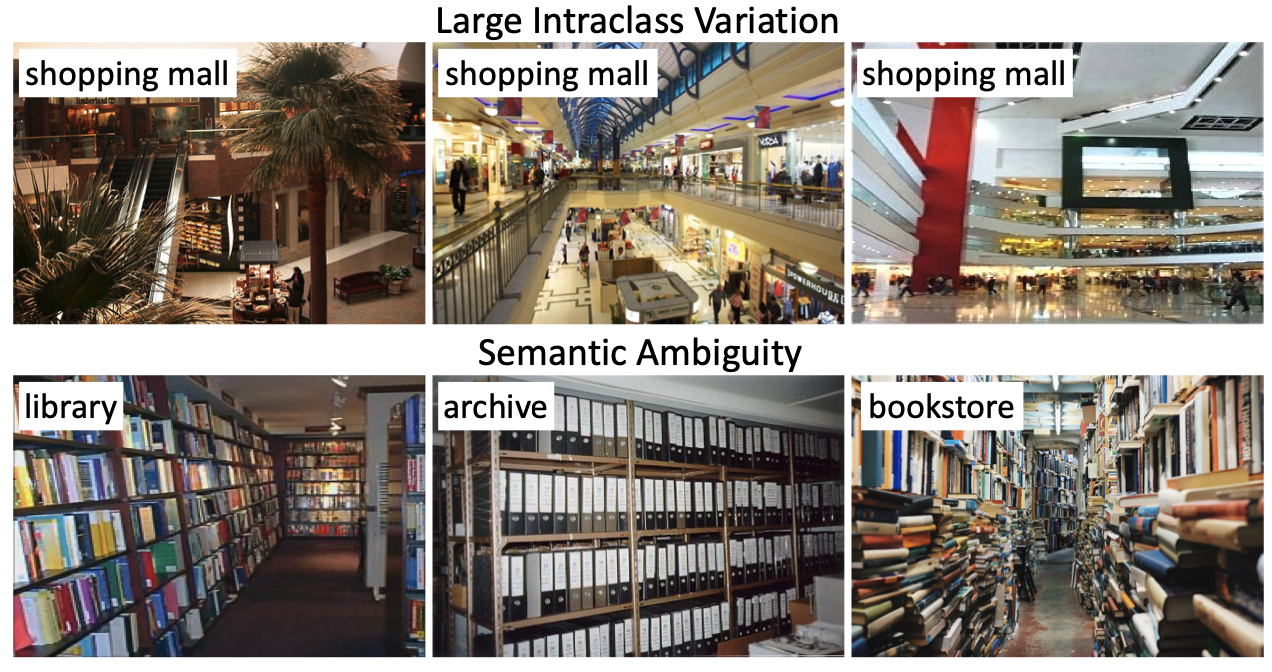
\includegraphics[width=\textwidth]{img/scene_class.png}
    \caption{Problem różnorodności wewnątrzklasowej oraz wieloznaczności semantycznej \cite{zeng2021deep}.}
    \label{fig:scene-class}
\end{figure}

Zadanie klasyfikacji sceny polega na przyporządkowaniu kategorii miejsca, które przedstawia obraz. Istnieje duża różnica między klasyfikacja obrazu a klasyfikacją sceny w kontekście trundości. Klasyfikacja obrazu jako taka zajmuje się przyporządkowaniem klasy obiektu pierwszoplanowego, np. czy na obrazie znajduje się pies, czy kot. Klasyfikacja sceny natomiast musi wziąć pod uwagę wszystkie cechy obrazu, zarówno tła, jak i pierwszego planu, by określić odpowiednie miejsce. 

W kontekście środowisk wewnętrznych klasyfikacja scen stanowi wyzwanie ze względu na zmienność scen wewnętrznych, obecność okluzji oraz fakt, że ten sam typ sceny może wyglądać inaczej na różnych obrazach. Wyróżniamy między innymi problem różnorodności wewnątrz klasowej oraz wieloznaczności semantycznej, co zostało przedstawione na rys. \ref{fig:scene-class}. Pierwszy z nich polega na fakcie, iż jedno miejsce może zostać przedstawione w bardzo różnej konfiguracji m.in. oświetlenia, ekspozycji, obiektów znajdujących się na obrazie. Drugi jest związany z występowaniem tych samych obiektów dla różnych klas scen.

\subsubsection{Segmentacja obrazu}
\begin{figure}[ht!]
    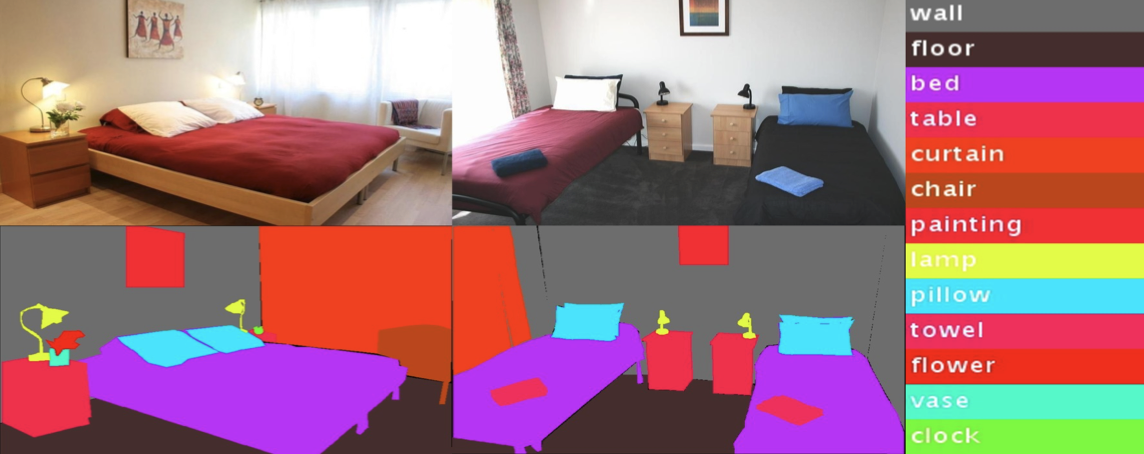
\includegraphics[width=\textwidth]{img/segment.png}
    \caption{Segmentacja wewnątrz pomieszczeń \cite{zhang2018context}.}
    \label{fig:segment}
  \end{figure}
  
Zadanie segmentacji obrazu to przyporządkowanie każdemu pikselowi etykiety takiej jak ,,łóżko'', ,,kanapa'' lub ,,umywalka'', do każdego piksela w obrazie (rys. \ref{fig:segment}). W rezultacie obraz zostaje podzielony na homogeniczne regiony pod względem pewnych własności. Segmentacja może być reprezentowana jako tablica 2D, gdzie każdy element odpowiada pikselowi w obrazie wejściowym i ma wartość wskazującą jego etykietę klasy.

Zadanie segmentacji można rozszerzyć do zadania segmentacji instancji (ang. instance segmentation), czyli segmentacji klasycznej rozszerzonej o rozróżnienie poszczególnych obiektów w ramach tej samej klasy. W przypadku klasycznej wersji nie jesteśmy w stanie rozróżnić dwóch stojących obok siebie łóżek, gdyż mapa segmentacji jest dla nich jednakowa. Segmentacja instancji pozwala natomiast takie rozróżnienie uczynić. Segmentacja semantyczna w dalszej części pracy będzie odnosić się do klasycznej wersji. Segmentacja instancji nie jest tematem pracy.
% # TODO: Zamienić obrazki definicji klasyfikacji i segmentacji na te z mojego zbioru

\subsection{Nadzorowane uczenie maszynowe}

Uczenie maszynowe jest częścią sztucznej inteligencji, które umożliwia przeprowadzanie wnioskowania z danych. Algorytmy te rozpoznają wzorce i dokonują przewidywań.

Uczenie nadzorowane to rodzaj uczenia maszynowego, w którym algorytm jest szkolony na etykietowanym zestawie danych, gdzie pożądane wyjście dla danego wejścia jest już znane. W kontekście głębokiego uczenia się, algorytmy uczenia nadzorowanego wykorzystują sieci neuronowe do uczenia się z danych i dokonywania przewidywań.

Jedną z głównych zalet wykorzystania głębokiego uczenia do uczenia nadzorowanego jest możliwość uczenia się złożonych i nieliniowych zależności wynikających z danych. Głębokie sieci neuronowe, z ich wieloma warstwami, mogą uczyć się i reprezentować wielowymiarowe i abstrakcyjne cechy danych, co pozwala im osiągnąć satysfakcjonujące rezultaty w wielu zadaniach. Co więcej, algorytmy głębokiego uczenia mogą obsługiwać duże ilości danych i mogą być łatwo zrównoleglone, co pozwala na skrócenie czasu treningu.

Istnieją jednak również ograniczenia w stosowaniu głębokiego uczenia do uczenia nadzorowanego. Jednym z ograniczeń jest konieczność posiadania dużej ilości oznaczonych danych. Aby wytrenować głęboką sieć neuronową, wymagana jest ich znaczna ilość. Dane nie zawsze mogą być łatwo dostępne lub łatwe do uzyskania. Co więcej, algorytmy głębokiego uczenia są często podatne na niskie obciążenie lub wysoką wariancję, zwłaszcza gdy ilość i jakość danych jest ograniczona. Może to prowadzić do słabej generalizacji.
\subsection{Głębokie uczenie i konwolucje}
Uczenie głębokie odnosi się do uczenia maszynowego, które charakteryzuje się wykorzystaniem głębokich sieci neuronowych. Składają się one z wielu warstw sztucznych neuronów. W kontekście wizji komputerowej głębokie uczenie jest wykorzystywane do skutecznego rozwiązywania wielu zadań, w tym klasyfikacji obrazów, wykrywania obiektów czy segmentacji semantycznej.

Jedną z kluczowych zalet głębokiego uczenia w wizji komputerowej jest zdolność do automatycznego uczenia się hierarchicznych reprezentacji obrazów. Wykorzystuje je się do wyodrębnienia wysokopoziomowych cech, które są wysoce zróżnicowane dla danego zadania. Stanowi to kontrast do tradycyjnych metod widzenia komputerowego, które zazwyczaj opierają się na ręcznie opracowanych cechach.

\subsection{Rozwój klasyfikacji obrazów}
Jedną z najwcześniejszych i najbardziej wpływowych prac w dziedzinie głębokich splotowych sieci neuronowych (CNN) jest ,,ImageNet Classification with Deep Convolutional Neural Networks'' autorstwa Alexa Krizhevsky'ego et al. (2012)\cite{krizhevsky2017imagenet}. W pracy tej przedstawiono zastosowanie głębokich sieci neuronowych do klasyfikacji obrazów i osiągnięto najwyższej wyniki na zbiorze danych ImageNet. Praca ta wyznaczyła nowy punkt odniesienia dla klasyfikacji obrazów i zapoczątkowała szerokie zastosowanie CNN w zadaniach widzenia komputerowego.

W kolejnych latach wielu badaczy zaproponowało różne modyfikacje i ulepszenia podstawowej architektury CNN. Jednym z ważnych wkładów jest architektura Inception, wprowadzona przez Szegedy et al. w ,,Going Deeper with Convolutions'' (2015)\cite{szegedy2015going}. Architektura Inception wykorzystuje kombinację różnych rozmiarów filtrów konwolucyjnych do ekstrakcji cech w wielu skalach, co pozwala sieci uczyć się bardziej złożonych i abstrakcyjnych cech niż wcześniejsze architektury.

Kolejną ważną innowacją było wykorzystanie połączeń rezydualnych, które zostało zaproponowane przez He et al. w ,,Deep Residual Learning for Image Recognition'' (2016)\cite{he2016deep}. Połączenia rezydualne pozwalają na trenowanie znacznie głębszych sieci, zapobiegając problemowi zanikających gradientów. Tak jak przedtem ImageNet posłużył do wykazania zalet tego rozwiązania.

Podsumowując, głębokie CNN są wysoce efektywne w zadaniach widzenia komputerowego, takich jak klasyfikacja obrazów. Rozwój głębokich CNN zaznaczył się kilkoma ważnymi kamieniami milowymi, takimi jak stosowanie różnych filtrów splotowych oraz wykorzystaniem połączeń rezydualnych. Te innowacje doprowadziły do znacznej poprawy wydajności na zbiorze danych ImageNet i zainspirowały dalsze badania w innych zadaniach widzenia komputerowego.
\subsection{Rozwój segmentacji semantycznej}
Jednym z najwcześniejszych i najbardziej wpływowych artykułów w dziedzinie głębokich CNN do segmentacji semantycznej jest ,,Fully Convolutional Networks for Semantic Segmentation'' autorstwa Longa, Shelhamera i Darrella (2015)\cite{fcn}. W pracy tej, zaprezentowanej na konferencji Computer Vision and Pattern Recognition (CVPR), przedstawiono architekturę sieci w pełni splotową (FCN) do segmentacji semantycznej. Architektura FCN wykorzystuje serię warstw splotowych i upsamplingu do produkcji gęstych predykcji per-piksel. Praca ta pokazała, że CNN mogą być wykorzystane do predykcji na poziomie pikseli i stworzyła podstawy dla wielu późniejszych podejść do segmentacji semantycznej.

Innym kluczowym wkładem w dziedzinie segmentacji semantycznej jest ,,U-Net: Convolutional Networks for Biomedical Image Segmentation'' autorstwa Ronneberger, Fischer i Brox (2015)\cite{ronneberger2015u}. W pracy tej, zaprezentowanej na międzynarodowej konferencji Medical Image Computing and Computer-Assisted Intervention (MICCAI), przedstawiono architekturę U-Net do segmentacji obrazów biomedycznych. Architektura U-Net wykorzystuje kombinację warstw splotowych i poolingowych do ekstrakcji cech w wielu skalach oraz serię warstw upsamplingu do produkcji gęstych predykcji per-piksel. Praca ta pokazała, że architektura U-Net dzięki zastosowaniu połączeń pomijających (skipping connections) jest w stanie znacznie lepiej rekonstruować obraz. Szczególnie dotyczy to elementów małej skali, które wcześniej były pomijane przez FCN. Praca ta została szeroko wykorzystana w obrazowaniu medycznym i nie tylko.

Kolejną ważną pracą w dziedzinie segmentacji semantycznej jest ,,DeepLab: Semantic Image Segmentation with Deep Convolutional Nets, Atrous Convolution, and Fully Connected CRFs'' autorstwa Chen, Papandreou, Kokkinos, Murphy i Yuille (2016)\cite{deeplab}. W pracy tej, zaprezentowanej na International Conference on Computer Vision (ICCV), przedstawiono architekturę DeepLab do segmentacji semantycznej. Architektura DeepLab wykorzystuje rozszerzony splot (atrous convolution) do zwiększenia pola widzenia warstw splotowych oraz warunkowe pola losowe (CRF) do dopracowania predykcji. Praca ta pokazała, że użycie rozszerzonego splotu i CRF może poprawić efekty segmentacji semantycznej.

Podsumowując, segmentacja semantyczna jest zadaniem o dużym znaczeniu w wizji komputerowej, a głębokie CNN okazały się wysoce skuteczne w rozwiązywaniu tego zadania. Rozwój głębokich CNN do segmentacji semantycznej został oznaczony przez kilka ważnych kamieni milowych, w tym wprowadzenie FCN przez Long et al., U-Net przez Ronneberger et al. i DeepLab przez Chen et al. Te architektury wyznaczyły nowe standardy w segmentacji semantycznej i zostały szeroko przyjęte w różnych dziedzinach zastosowań.


% \subsection{DeepLabV3}
% Literatura uważa go za model lepszy od sieci U-Net czy FCN. Model DeepLabV3 (rys. \ref{fig:deeplabv3}) nie korzysta z połączeń pomijających. Informacje o kontekście w wielu skalach uzyskuje przez moduł Spatial Pyramid Pooling (SPP). Wykorzystuje on bloki Atrous Spatial Pyramid Pooling (ASPP) oraz klasyczny pooling. Bloki ASPP składają się ze splotu, normalizacji pakietowej oraz funkcji aktywacji ReLU. Sploty przyjmują różną postać. Pierwszy blok to splot o jądrze 1x1. Następne bloki korzystają z rozszerzonego splotu o dylatacji oraz wypełnieniu (padding) równemu współczynnikowi rozszerzenia (dilatation rate). Dla kolejnych 3 bloków wynosi on 12, 24, 36. Ostatni blok SPP to zwykły pooling. Bloki składające się na moduł SPP są następnie dodawane wzdłużnie i poddawane splotowi. Następnie egzekwuje się splot o wyjściowej liczbie kanałów równej ilości klas. Końcowy etap obejmuje upsampling do pożądanego wymiaru.
% \begin{figure}[ht!]
% 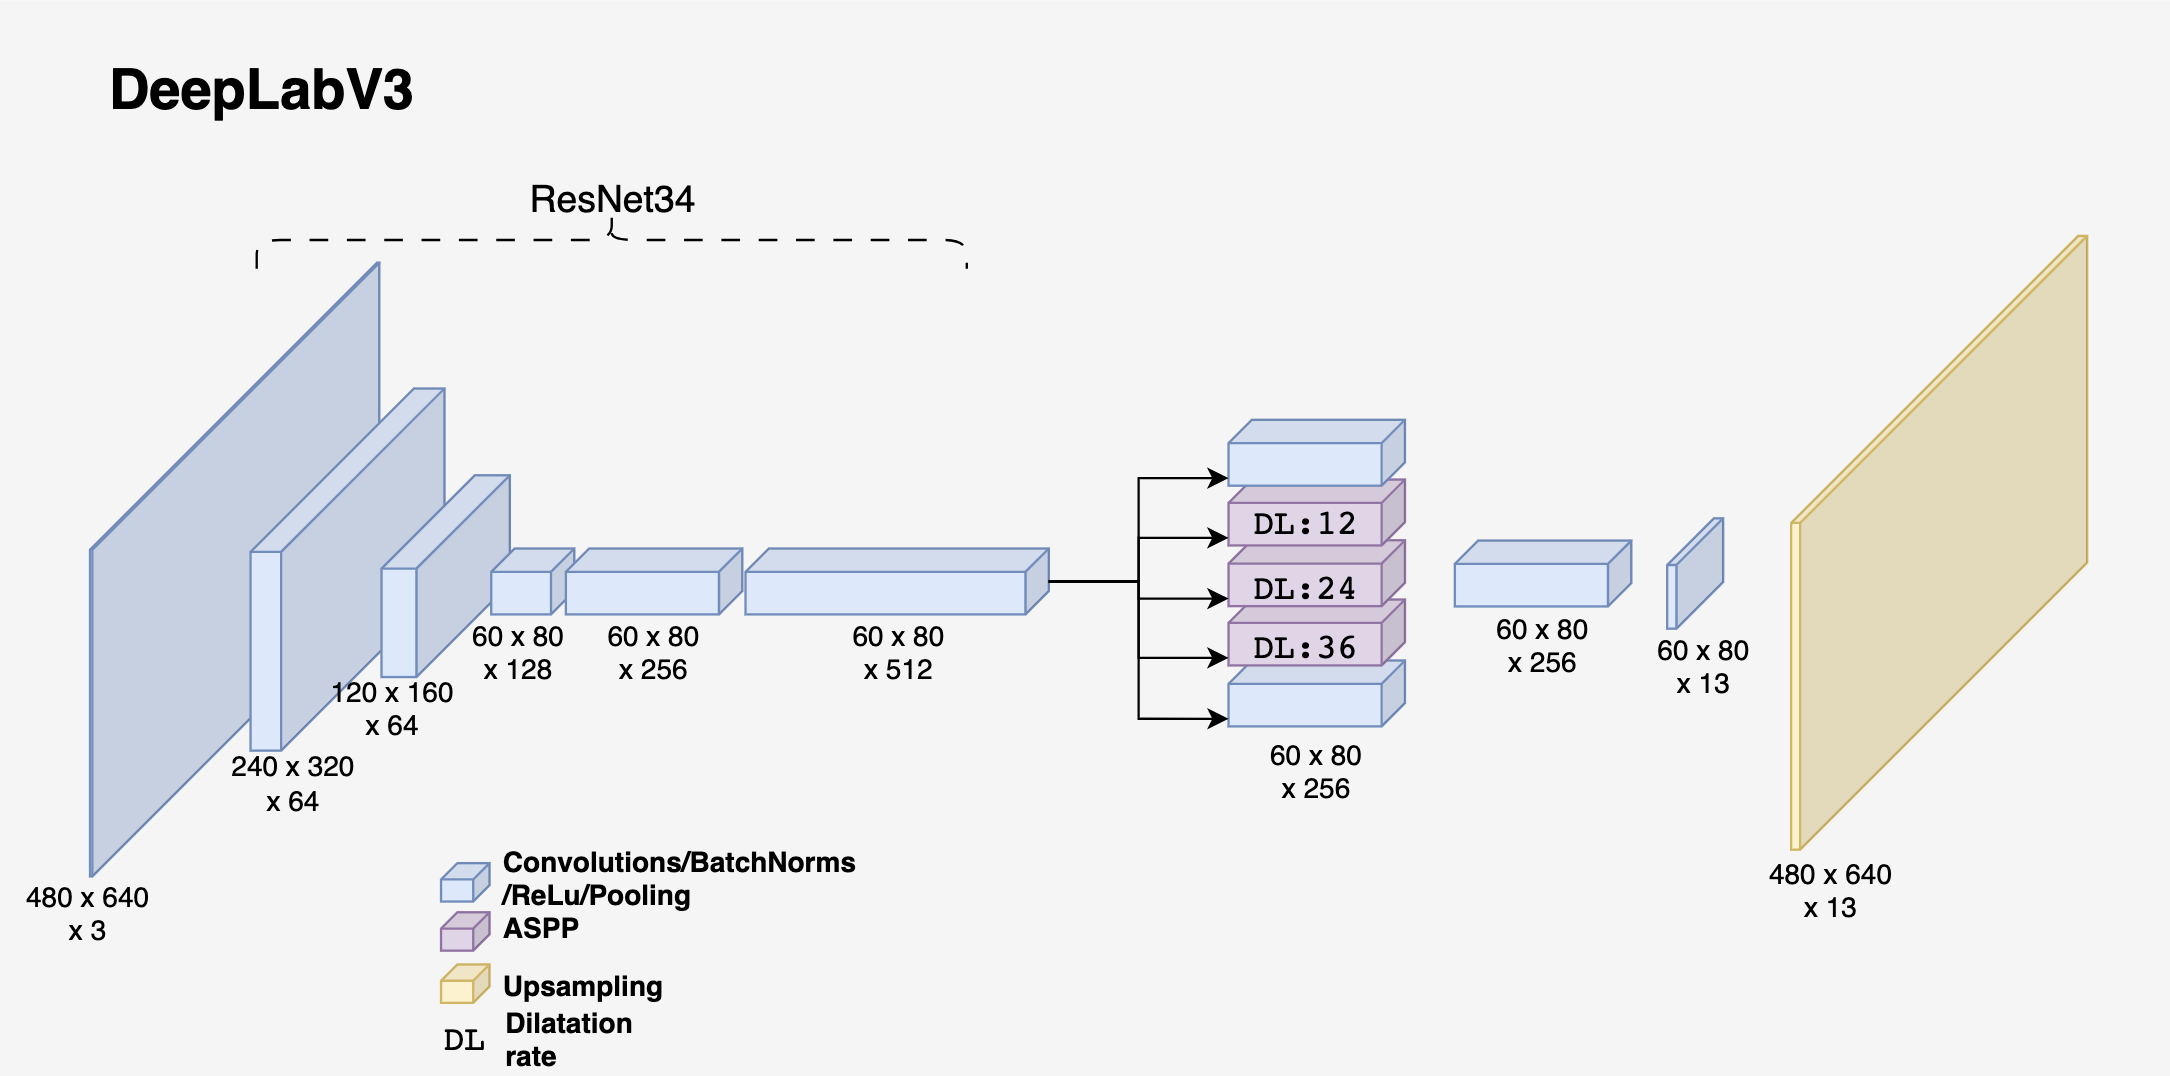
\includegraphics[width=\textwidth]{deeplabv3-new.png}
% \caption{Klasyczna architektura DeepLabV3 z backbonem ResNet34.}
% \label{fig:deeplabv3}
% \end{figure}

\subsection{Finetuning}
Finetuning jest metodą uczenia głębokich sieci neuronowych. Polega on na odtworzeniu wag modelu, wcześniej wytrenowanego na dużym zbiorze danych jak ImageNet, a następnie próbie dostosowania go do obecnie rozważanego problemu. W kontekście wizji komputerowej pierwsze warstwy modelu są najczęściej ogólne i odnoszą się do generalnych cech obrazu. Ta wiedza pozwala wnioskować, że pierwsza część modelu nie zależy w głównej mierze od zbioru danych oraz rozważanego zadania, tylko jest czymś ogólnym dla wielu problemów przetwarzania obrazu. Zatem pojawia się możliwość ponownego użycia część gotowego modelu. W takim przypadku mowa o transferze wiedzy. Technicznie finetuning najczęściej rozpoczyna się od uczenia modelu, wykorzystując jedynie ostatnie warstwy. W miarę kolejnych epizodów uczenia wykorzystuje się coraz więcej warstw sieci. Taki zabieg nazwy się odmrażaniem kolejnych warstw sieci.
\subsection{Uczenie wielozadaniowe}
Uczenie wielozadaniowe jest techniką uczenia maszynowego, w której model jest trenowany do wykonywania wielu zadań jednocześnie. Zabieg ten stosuje się w celu nauczenia się wspólnych reprezentacji, które mogą poprawić skuteczność we wszystkich zadaniach. To podejście zyskało uwagę w ostatnich latach ze względu na rosnące zapotrzebowanie na modele, które mogą wykonywać wiele zadań z wysoką dokładnością i wydajnością. Uczenie wielozadaniowe ma szereg zastosowań, takich jak widzenie komputerowe, przetwarzanie języka naturalnego i rozpoznawanie mowy.

Sebastian Ruder w swoim przeglądzie literatury ,,An Overview of Multi-Task Learning in Deep Neural Networks'' (2017) \cite{ruder2017overview} dość zwięźle definiuje uczenie wielozadaniowe jako optymalizację co najmniej dwóch funkcji straty. Co więcej, pokazuje, że takie podejście ma swoje silne biologiczne analogie. Autor dopatruje się tutaj odpowiedzi na pytanie, czym jest uczenie się uczenia (learnig to learn), a więc główna przesłanka bardzo silnego nurtu meta-learningu. Podkreśla, że uczenie wielozadaniowe pomaga osiągać lepsze rezultaty niż klasyczne uczenie jednego zadnia. Zachęca nawet do stosowania uczenia wielozadaniowego w przypadku, gdy potrzebujemy zaledwie jednego zadania poprzez znalezienie zadania lub zadań komplementarnych. Autor wielokrotnie odwołuje się do dzieła ,,Multitask learning: A knowledge-based source of inductive bias'' (1993) \cite{caruana1993multitask} przypominając, że uczenie wielozadaniowe przyczynia się do lepszej generalizacji modelu, a więc uniezależnienie się od domeny uczącej na rzecz szeroko pojętej wiedzy.

Ruder opisuje dwa główne podejścia do uczenia wielozadaniowego — twarde oraz miękkie dzielenie wag sieci (soft/hard parameter sharing). Twarde dzielenie wag jest najczęściej stosowane. Polega na uwspólnieniu pierwszej części sieci, odpowiedzialnej za zdefiniowanie przestrzeni reprezentacji (ang. backbone) oraz rozdzieleniu kolejnych warstw związanych z konkretnym zadaniem. Miękkie dzielenie wag polega na zbudowaniu wielu sieci, odpowiednich dla danego zadania. Co więcej, sieci te podczas uczenia są regularyzowane w ten sposób, aby zachęcić je do posiadania jak najpodobniejszych wag.

Takie podejście może się powieść jedynie w przypadku, kiedy dwa zadania są powiązane ze sobą. Powstało wiele prac poświęconych odpowiedzi na pytanie, które zadania warto wybrać, a które należy rozpatrywać osobno. Jednym z takich dzieł jest praca zespołu ze Stanfordu ,,Which Tasks Should Be Learned Together in Multi-task Learning?'' Standley et al. (2020) \cite{standley2020tasks}. Przedstawia ona pojęcie negatywnego wpływu (ang. negative transfer), który najprościej rzecz ujmując sprawia, że sieć uczy się gorzej niż pojedyncze sieci. Autorzy zbadali, że największy wpływ na jakość uczenia wielozadaniowego ma właśnie odpowiedni dobór zadań, a niekoniecznie rozmiar zbioru danych czy wielkość modelu. Oczywiście należy zwrócić uwagę, że przytoczone czynniki nie są bez znaczenia, jedynie w porównaniu z doborem zadań mają pomijalne znaczenie. Co ciekawe zadania afiniczne względem siebie mogą mieć dodatni wpływ w przypadku transferu wiedzy, a nie muszą być afiniczne w kontekście uczenia wielozadaniowego.

Gdy jednak zadania są pokrewne względem siebie, jesteśmy w stanie zaobserwować konkretne korzyści związane ze wspólnym uczeniem. Ruder wymienia kilka najważniejszych. Po pierwsze zyskujemy tak zwaną bezpośrednią augmentację danych (ang. implicit data augmentation). Każde z zadań posiada pewien szum związany z konkretnym zadaniem. Uczenie wielu zadań pozwala w pewnym stopniu wyeliminować szum związany z konkretnym zadaniem na rzecz lepszej generalizacji. Kolejną zaletą jest lepsze skupienie uwagi na ważnych informacjach. Ma to szczególne znaczenie w przypadku gdy dane są ograniczone lub wielowymiarowe. Uczenie wielozadaniowe może pomóc w wyborze tych najbardziej znaczących cech. Co więcej, wspólna wiedza zdobyta podczas uczenia może okazać się znacząca. Niektóre cechy są łatwiejsze do wykrycia dla jednego zadania, inne dla drugiego. Łącząc te informacje przez tak zwane ,,podsłuchiwanie'' (ang. eavesdropping) model jest w stanie zbudować lepszą przestrzeń reprezentacji. Oprócz zyskania na jakości modelu przypadek twardego dzielenia wag pozwala znacząco ograniczyć wielkość modelu. Nie trzeba bowiem stosować wielu backbone'ów, które stanowią największą część modelu w kontekście liczby parametrów. Implikuje to znacznie zmniejszenie czasu uczenia oraz wnioskowania \cite{standley2020tasks}.
\newpage % Rozdziały zaczynamy od nowej strony.
\section{Rozwiązanie}

W tym rozdziale przedstawione zostaną wybrane metody, które zostały sprawdzone w ramach analizy problemu. Rozważania zostaną przedstawione w ścisłym związku z pytaniami badawczymi przedstawionymi w celu pracy, a więc:

\begin{itemize}
    \item Jak można zaprojektować model oparty na głębokim uczeniu do wspólnej segmentacji semantycznej i klasyfikacji scen w środowiskach wewnętrznych?
    \item Czy przestrzeń reprezentacji po wytrenowaniu na zadaniu segmentacji semantycznej może być użyta do zadania klasyfikacji sceny?
    \item Jak dobrze proponowany model radzi sobie na dużym zbiorze danych scen wewnętrznych i jak wypada w porównaniu z aktualnymi metodami segmentacji semantycznej i klasyfikacji scen osobno?
    \item Jak proponowany model może być wykorzystany do poprawy wydajności w robotyce mobilnej?
\end{itemize}
Opis rozwiązań problemu zostanie poprzedzony przeglądem rozwiązań. Analiza dotychczasowego stanu wiedzy pozwoli lepiej ukierunkować badania. Intuicja oraz wskazówki zdobyte podczas przeglądu zostaną uwzględnione w doborze metod i eksperymentów.

\subsection{Przegląd rozwiązań}
Przegląd literatury jest kluczowym aspektem każdej pracy naukowej. W tym podrozdziale zostaną przedstawione wyłącznie rozwiązania obejmujące łączną segmentację semantyczną oraz klasyfikację sceny. Szczególny nacisk położony zostanie na architektury głębokich, wielozadaniowych sieci neuronowych. Niestety przyjęte założenia w pracy nie zostały opisane przez nikogo wcześniej, zgodnie z najlepszą wiedzą autora. Niektóre prace naukowe przedstawiają ten sam problem, to jest klasyfikacji i segmentacji łącznie, ale obejmują go w innej domenie danych. Z drugiej strony artykuły obejmujące środowiska wnętrz są dobrze zdefiniowane, jednak często w swoich rozwiązaniach autorzy korzystają z obrazu głębi, który nie zawiera się w zakresie badań tej pracy. Nie mniej wszystkie poniższe artykuły stanowią cenne źródło informacji oraz wskazówek.

\vspace{0.5cm}

Pierwszym z prezentowanych artykułów jest ,,Describing the Scene as a Whole: Joint Object Detection, Scene Classification and Semantic Segmentation'' autorstwa Yao J. et al. (2012)\cite{yao2012describing}. Prezentuje on algorytm, który ówcześnie wyznaczył najlepsze podejście (ang. state-of-the-art (SOTA)). Rozwiązanie opiera się na warunkowych polach losowych, które ówcześnie były szeroko stosowane. Mimo że nie jest to rozwiązanie oparte o głębokie sieci neuronowe, to autorzy wskazują tutaj ważne zagadnienia. Po pierwsze udowadniają, że połączenie segmentacji i klasyfikacji okazało się owocne nie tylko pod względem jakości, ale również wydajności w kontekście czasowym. W swojej pracy wykorzystują podejście równolegle zgodne z rysunkiem \ref{fig:scene-as-a-whole}. Podsumowując, ,,Describing the Scene as a Whole: Joint Object Detection, Scene Classification and Semantic Segmentation'' nie jest propozycją architektury głębokiej sieci. Wskazuje on na problemy z łączeniem zadań szeregowo, jednocześnie udowadniając, że taka praktyka był ówcześnie stosowana, więc nie można uznawać stosowania połączenia szeregowego jako niedopuszczalnego. Poza tym autorzy doceniają wspólne realizowanie zadań, oceniając je jako bardziej efektywne czasowo i obliczeniowo.

\begin{figure}[ht!]
    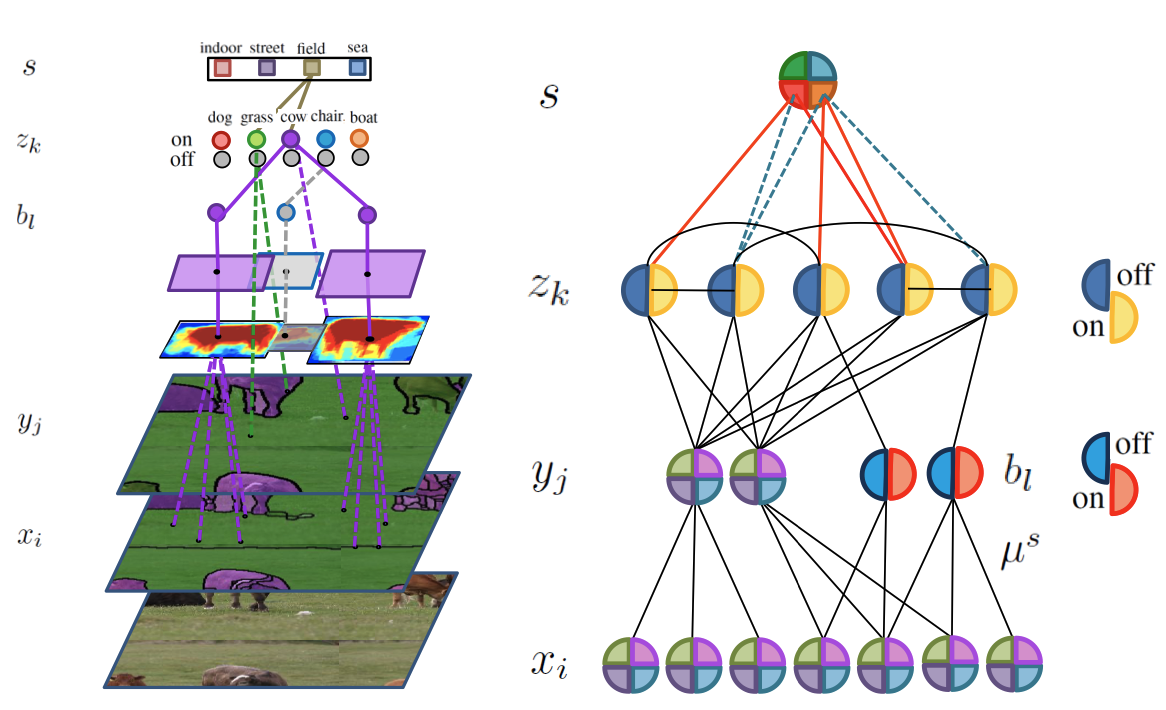
\includegraphics[width=\textwidth]{img/joint-segmentation-and-classification.png}
    \caption{Describing the Scene as a Whole: Joint Object Detection, Scene Classification and Semantic Segmentation (2012) \cite{yao2012describing}.}
    \label{fig:scene-as-a-whole}
\end{figure}
\vspace{0.5cm}
Artykuł ,,Let there be Color!: Joint End-to-end Learning of Global and Local Image Priors for Automatic Image Colorization with Simultaneous Classification'' (2016) \cite{iizuka2016let} przedstawia rozwiązanie problemu jednoczesnego klasyfikowania sceny oraz kolorowania zdjęć. Do realizacji zadania kolorowania potrzebna jest semantyczna maska. Wynika z tego, że kolorowanie jest rozszerzeniem segmentacji semantycznej. Rozumiejąc towarzyszące analogie, można przejść do analizy rozwiązania. Przedstawiona architektura (rys.\ref{fig:parrarel-arch}) jest przykładem sieci wielozadaniowej, używającej miękkiego dzielenia parametrów, ale tylko i wyłącznie w obrębie pierwszej części sieci. Szczególnie ciekawa jest konkatenacja cech wysokiego poziomu (Global Features Network) z cechami średniopoziomowymi (Mid-Level Features Network), która ma miejsce w warstwie fuzji (Fusion layer). Iizuka et al. formułują wniosek oznajmiający o kluczowym znaczeniu tej warstwy w kontekście całego zadania. Wiedza o scenie zdjęcia może dostarczyć informacji wpływających na decyzję, czy na obrazie znajduje się niebo, czy trawa. Rozważając sceny wnętrz, oczywiste jest, że nie będzie tam takich grup semantycznych, jednak bezpośrednia informacji o miejscu sceny, np. łazienka, może pomóc w ustaleniu etykiet segmentacji. Podsumowując, cechy nauczone na zadaniach klasyfikacji i segmentacji, mogą wzajemnie pozytywnie na siebie wpływać, realizując pozytywny transfer.
\begin{figure}[ht!]
    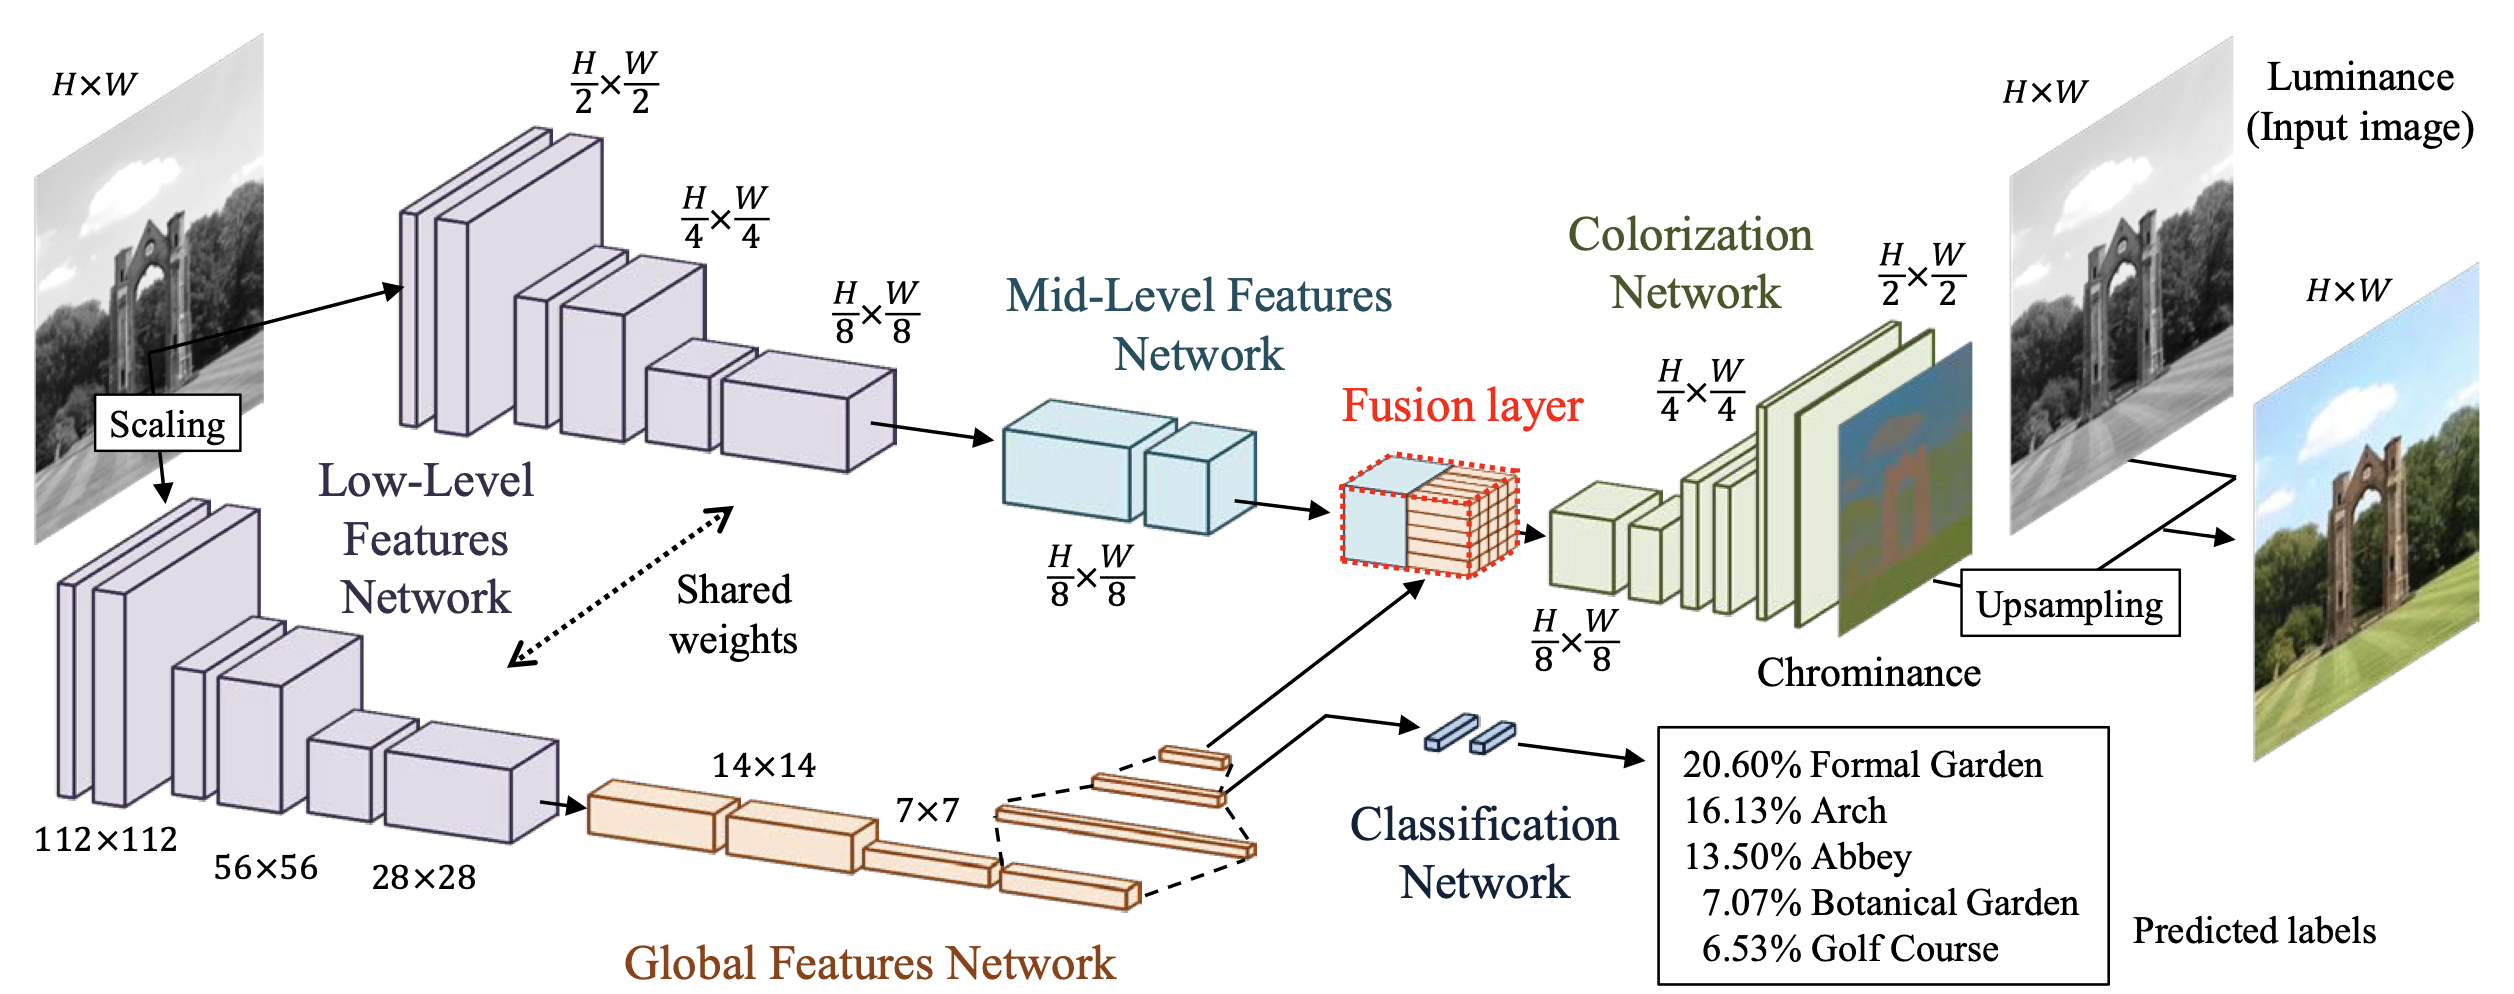
\includegraphics[width=\textwidth]{global-local-features.png}
    \caption{Let there be Color!: Joint End-to-end Learning of Global and Local Image Priors for Automatic Image Colorization with Simultaneous Classification 2016 \cite{iizuka2016let}.}
    \label{fig:parrarel-arch}
\end{figure}


\vspace{0.5cm}
Zastosowanie łącznej segmentacji oraz klasyfikacji tym razem w domenie obrazowania medycznego przedstawia ,,Y-Net: Joint Segmentation and Classification for Diagnosis of Breast Biopsy Images'' (2018) \cite{mehta2018net}. Zadania te są realizowane przez twarde dzielenie parametrów w kontekście uczenia wielozadaniowego (rys. \ref{fig:y-net}). Architektura jest prostym rozszerzeniem klasycznego U-Netu. Autorzy wskazują, że taki zabieg powoduje dużą modularność, ponieważ do dowolnego modelu segmentacji można podłączyć sieć klasyfikacyjną. Przeprowadzone eksperymenty dla segmentacji udowodniły, że dokładność pozostała na tym samym poziomie. W przypadku klasyfikacji wyniki były wyższe niż dotychczasowe SOTA na tym zbiorze. Jako funkcję straty autorzy użyli sumy entropii skrośnej każdego z zadań. Podsumowując, zadanie segmentacji osiągnęło ten sam wysoki wynik co SOTA, a zadanie klasyfikacji ustanowiło nowe SOTA na tym zbiorze, ucząc się znacznie mniej parametrów.


\begin{figure}[ht!]
    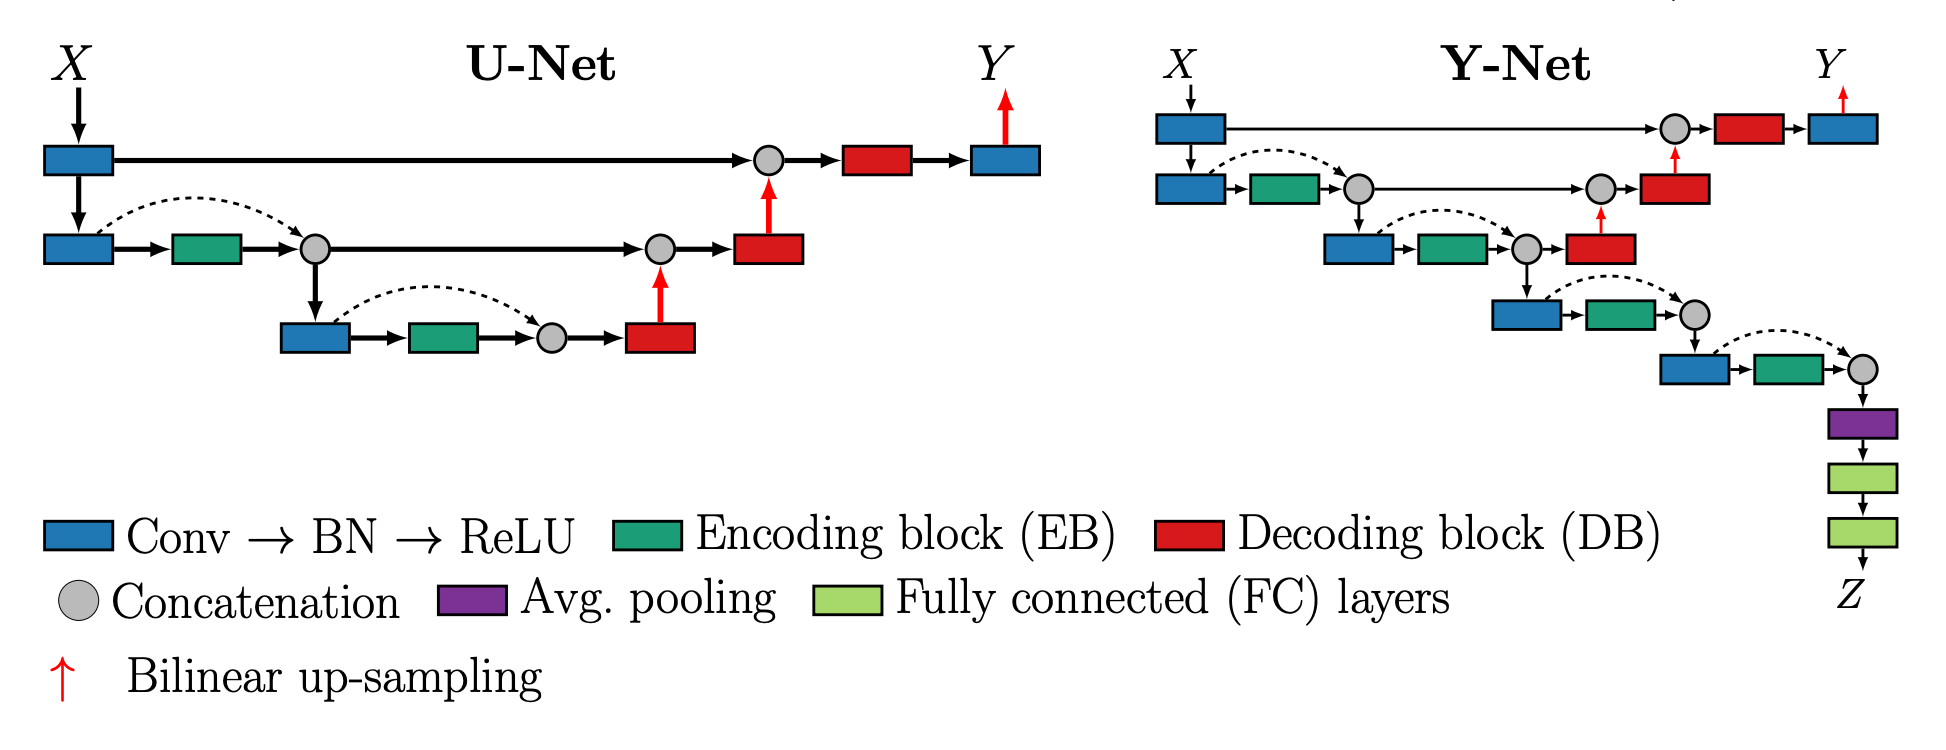
\includegraphics[width=\textwidth]{y-net-new.png}
    \caption{Y-Net: Joint Segmentation and Classification for Diagnosis of Breast Biopsy Images 2018 \cite{mehta2018net}.}
    \label{fig:y-net}
\end{figure}

\vspace{0.5cm}

Najbliższym artykułem tej pracy inżynierskiej jest ,,Efficient Multi-Task RGB-D Scene Analysis for Indoor Environments'' (2022) \cite{9892852}, który został opublikowany w czasie tworzenia tej pracy. Przedstawia on jedną głęboką sieć neuronową rozwiązującą następujące zadania: segmentacja semantyczna oraz segmentacja instancji (łącznie ang. pantopic segmentation), estymacja orientacji instancji oraz klasyfikacja sceny. Rozważaną przez autorów domeną są podobnie jak w przypadku tej pracy sceny wnętrz. Znaczną różnica poza dodatkowymi zadaniami jest użycie przez Seichter et al. informacji o głębi. Zgodnie z wnioskami z niniejszego artykułu przetwarzanie łączne obrazów RGB i głębi jest kluczowe z punktu widzenia jakości predykcji, więc nie można bezpośrednio porównać go z niniejszą pracą. Autorzy wykonali wiele eksperymentów, badając różne metodologie. Architektura jest przedstawiona na rysunku \ref{fig:emsanet}. Autorzy zdecydowali się na twarde dzielenie parametrów, argumentując całkowitą niezależnością w przypadku chęci wyłączenia jednego zadań z wnioskowania. Pierwszym krokiem, który wykonali, było ustalenie punktu odniesienia poprzez trenowanie osobno każdego z zadań. Trening każdej sieci z osobna był rozważany pod względem wielu backbone'ów ze zróżnicowaniem na uczenie wyłącznie obrazu głębi, obrazu RGB lub RGB-D. Z reguły w przypadku segmentacji oraz klasyfikacji większy backbone wpływał na polepszenie wyników. Trenując zadania łącznie, zdecydowano się na ważoną sumę entropii skrośnej dla zadania segmentacji i klasyfikacji w proporcjach odpowiednio 3:1. Przyjęty krok uczenia, będąc sprawdzonym przez przeszukiwanie liniowe (ang. grid search), jest wyjątkowo duży, bo wynosi 0.02. Autorzy zastosowali zaawansowane techniki dostosowywania kroku uczenia w trakcie treningu poprzez użycie planisty polityki jednego cyklu (ang. one cycle policy scheduler). Jako optymalizator użyto SGD z momentem oraz drobną regularyzacją. Podsumowując, zgodnie z prezentowanymi wynikami na wspólnej segmentacji oraz klasyfikacji autorom nie udało się polepszyć działania modelu na segmentacji semantycznej. Z powodzeniem jednak wzrosła dokładność klasyfikacji na zbiorze NYUv2.

\begin{figure}[ht!]
    \centering
    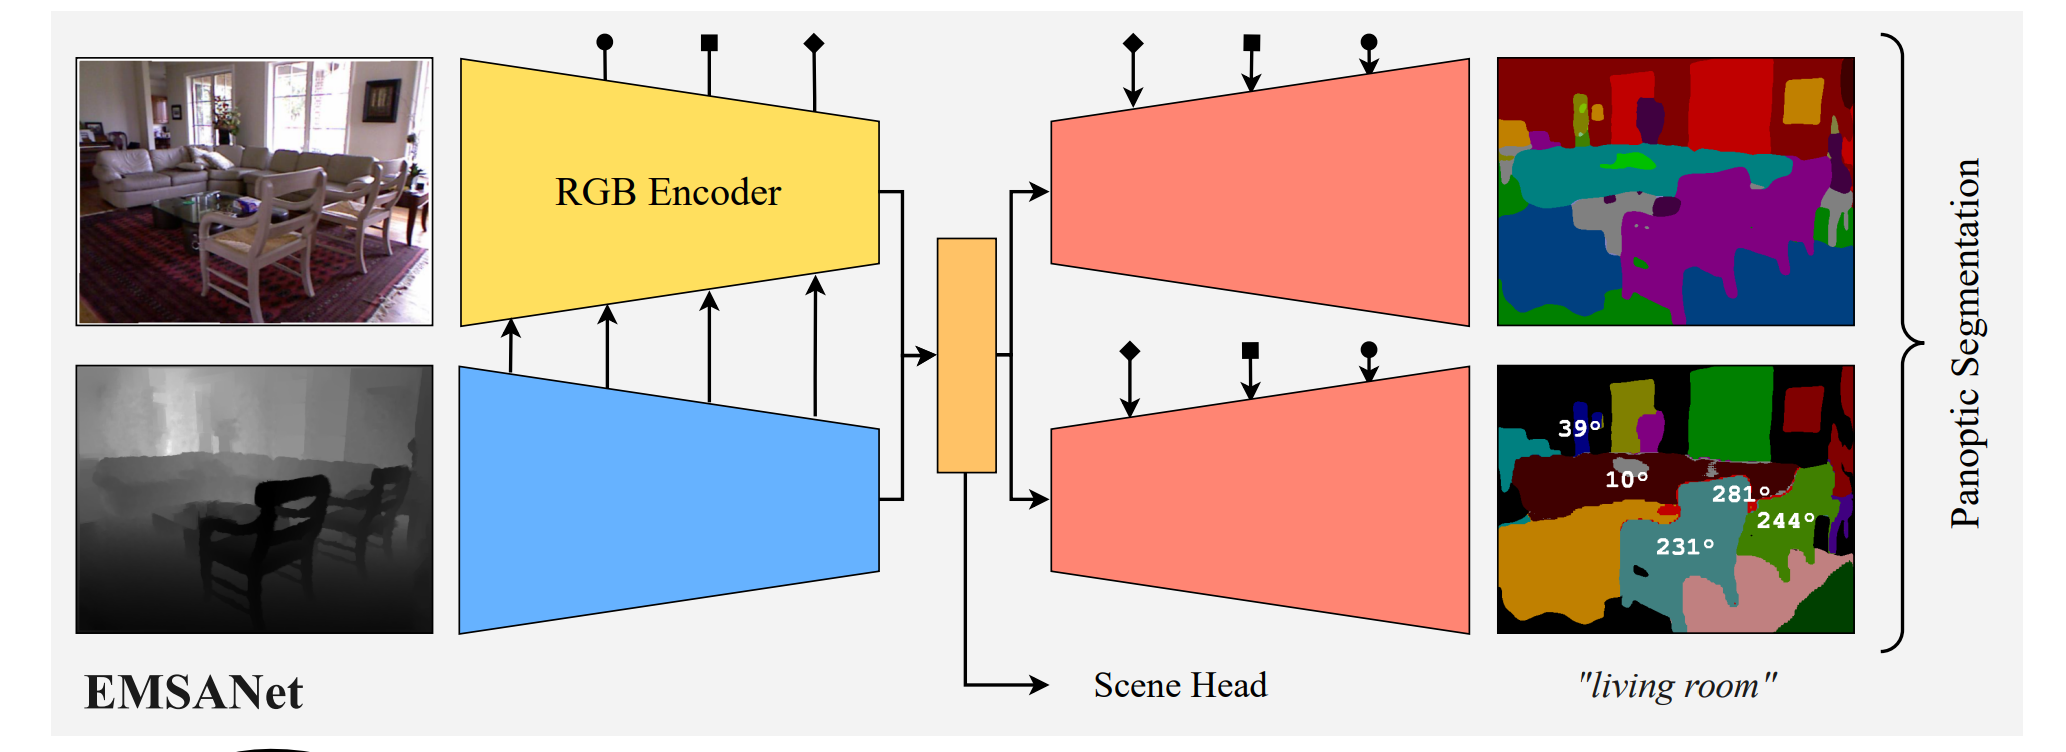
\includegraphics[width=\textwidth]{emsanet.png}
    \caption{Efficient Multi-Task RGB-D Scene Analysis for Indoor Environments \cite{9892852}}
    \label{fig:emsanet}
\end{figure}


\subsection{Rozwiązanie problemu}
W tym podrozdziale zostaną przedstawione eksperymenty, które wykonano w celu zbadania uczenia wielozadaniowego segmentacji semantycznej oraz klasyfikacji sceny w domenie pomieszczeń. Pierwszym etapem, jakiego dokonano, było wyznaczenie punktu odniesienia. Z punktu widzenia pracy najłatwiej byłoby znaleźć gotowe wyniki segmentacji oraz klasyfikacji sceny na wybranym zbiorze danych. Niestety żadne z przytaczanych rozwiązań nie odpowiada w pełni zakresowi pracy. Postanowiono stworzyć taki punkt odniesienia samemu przez analogiczne trenowanie sieci segmentacyjnej oraz klasyfikacyjnej osobno.

Mając taką wiedzę, eksperymentowano dalej z różnymi architekturami uczenia wielozadaniowego. Wybrano uczenie łączne o twardym dzieleniu parametrów. Podejście to ma wiele zalet. \cite{mehta2018net} podkreśla łatwość i wszechstronność implementacji. Wystarczy dołączyć do modelu część klasyfikacyjną. Co więcej, wszyscy autorzy (\cite{mehta2018net}, \cite{9892852}) chwalą znacznie mniejszą ilość parametrów sieci, co bezpośrednio wpływa na czas treningu oraz wnioskowania. Architektura sieci przedstawia rys. \ref{fig:multitask}. Jest to DeepLabv3 rozszerzony za enkoderem o sieć klasyfikacyjną podobnie jak w artykule \cite{mehta2018net}, gdzie rozszerzono sieć U-Net.

\begin{figure}[ht!]
\centering
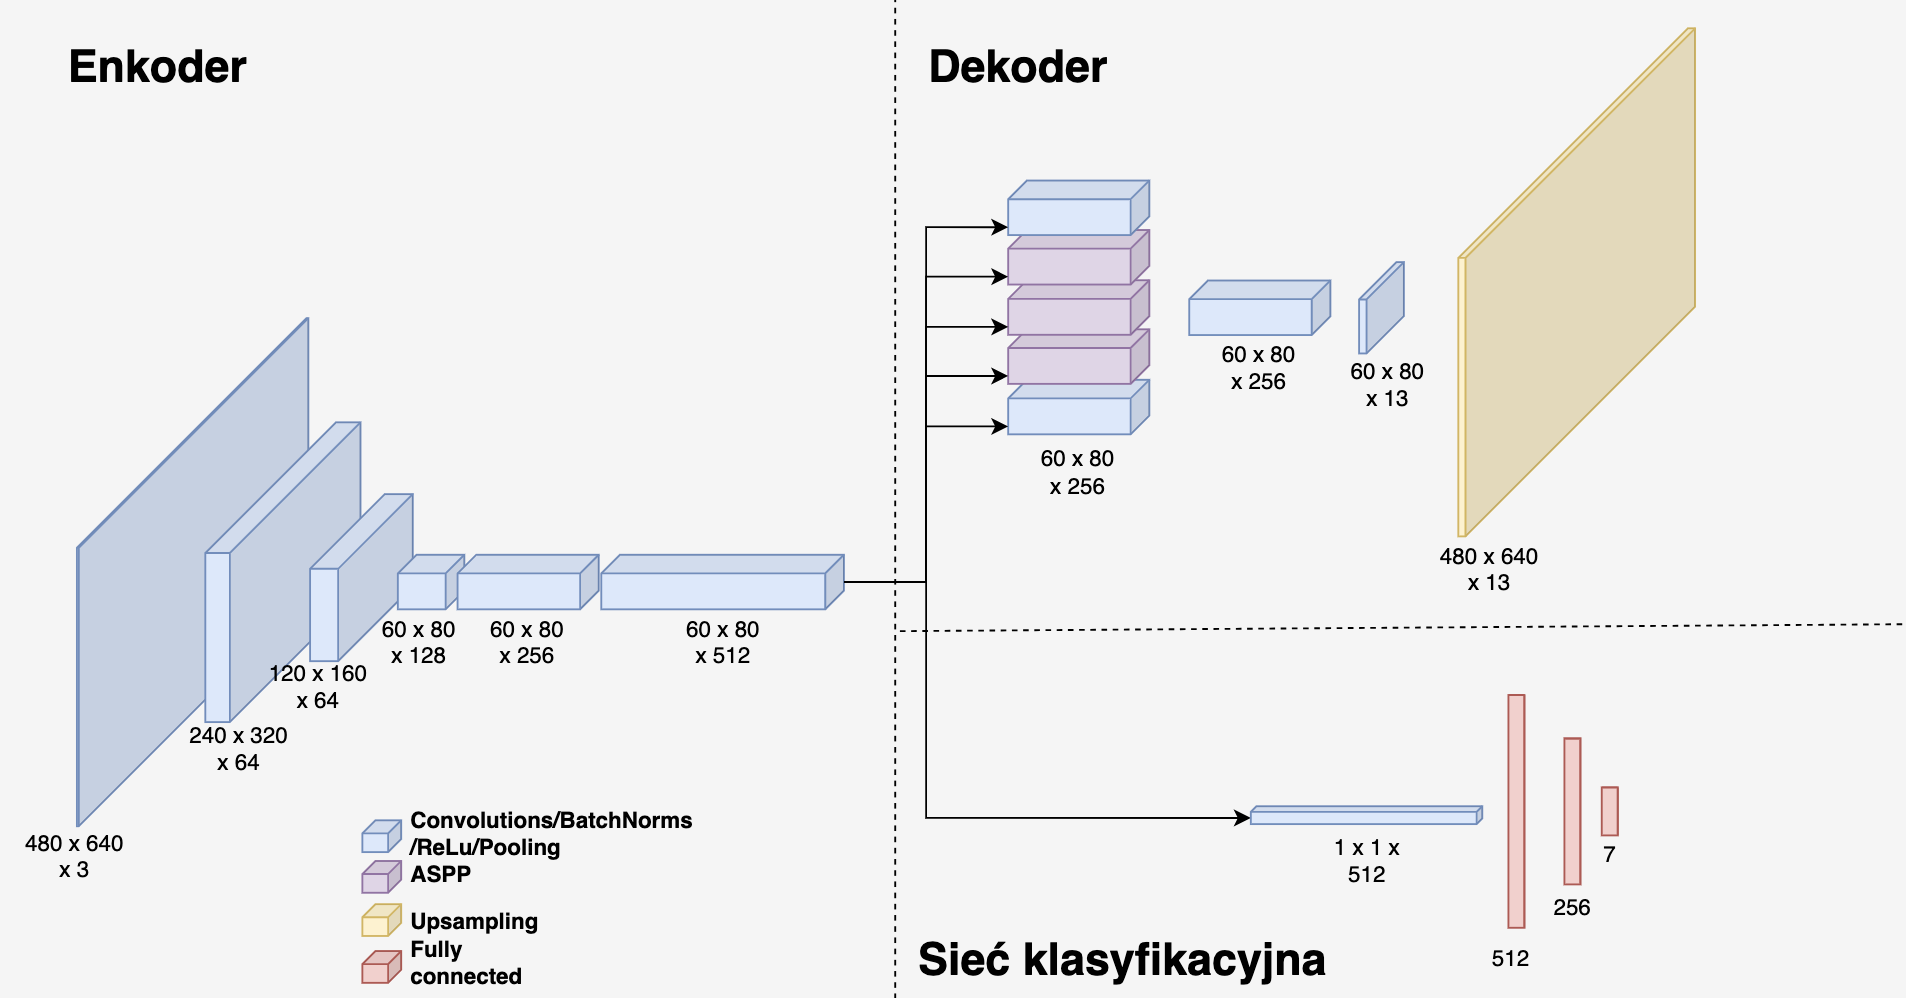
\includegraphics[width=\textwidth]{multitask-arch-new.png}
\caption{Architektura wielozadaniowej sieci.}
\label{fig:multitask}
\end{figure}

Normalizacja jest ważnym krokiem przetwarzania wstępnego w problemach widzenia komputerowego. W pracy ,,Normalization Techniques in Training DNNs: Methodology, Analysis and Application'' Lei et. al. \cite{huang2020normalization}, autorzy udowadniają, że normalizacja stabilizuje i przyśpiesza trening oraz prawdopodobnie prowadzi do poprawy generalizacji. Jako przetwarzanie wstępne obrazu zastosowano normalizację gaussowską. Obrazy RGB zostały poddane normalizacji ze średnią (0.485, 0.456, 0.406) oraz odchyleniem standardowym (0.229, 0.224, 0.225), które odpowiadają parametrom rozkładu normalnego na zbiorze ImageNet. Gotowe wagi uzyskane poprzez uczenie na bazie ImageNet służyły jako wagi początkowe enkodera.

Znalezienie optymalnego zestawu hiperparametrów nie jest proste. Niewłaściwy dobór grozi brakiem osiągnięcia pożądanych rezultatów. W celu pozyskania optymalnego zestawu skorzystano z narzędzia Optuna \cite{optuna_2019}. Wykorzystano do tego algorytm TPE (Tree-structured Parzen Estimator), który jest znacznie korzystniejszy niż klasyczne przeszukiwanie siatką (Grid Search). Optymlaizacja hiperparametrów nie tylko poprawia łatwość doboru hiperparametrów, ale przede wszystkim podwyższa wiarygodność rezultatów. Hiperparametry były optymalizowane względem straty na zbiorze walidacyjnym. Do optymalizowanych parametrów zalicza się tylko krok uczenia, chyba że stwierdzono w dalszej części rozdziału inaczej.

Do klasycznych funkcji straty dla segmentacji semantycznej zaliczamy entropię skrośną, ale również coraz popularniejsze Lov\'asz Softmax \cite{berman2018lovasz} czy Focal Loss \cite{jadon2020survey}. Entropia i Focal jest stratą związaną z dystrybucją pikseli, Lov\'asz Softmax skupia się bardziej na konkretnych regionach \cite{jadon2020survey}. W przypadku zadania klasyfikacji najczęściej spotykana jest entropia skrośna. W pracy wykorzystano entropię skrośną zarówno dla klasyfikacji, jak i dla segmentacji semantycznej podobnie jak \cite{mehta2018net} oraz \cite{9892852}. Entropia była ważona poprzez odwrotność sumy odpowiednio pikseli dla danej etykiety semantycznej oraz etykiet związanej ze scenami.

Samo uczenie nie było długie, bo trwało od 5 do 15 epok. Zastosowano wczesne przerwanie treningu (Early Stopping), monitorując stratę na zbiorze walidacyjnym, by uniknąć przeuczenia. Poza tym zastosowano zmienny krok uczenia poprzez planistę typu ekspotencjalnego (exponential learnig rate policy) o współczynniku $\gamma$ równemu 0.99, który zmniejsza krok uczenia o $\gamma$ co epokę.

W dalszej części przedstawione zostaną konkretne eksperymenty, które rozważano w pracy.

\subsubsection{Uczenie wielozadaniowe}
Uczenie wielozadaniowe zostało zrealizowane przez architekturę z rysunku \ref{fig:multitask}. Trening polegał na aktualizowaniu wag całego dostępnego modelu zgodnie z propagacją wsteczną agregowanej funkcji straty $\lambda$. Zaimplementowano ją jako sumę funkcji strat na każdym z zadań tak jak w przypadku \cite{mehta2018net}. Nie stosowano ważenia zadań wspomnianego w \cite{9892852}. Ważenia zadań nie należy mylić z ważeniem etykiet w funkcji straty
\begin{equation*}
\lambda = \lambda_{segmentacja} + \lambda_{klasyfikacja}
\end{equation*}

\subsubsection{Wyłącznie klasyfikacja}
W celu określenia punktu odniesienia wytrenowano model, zapominając o podsieci do wyznaczania segmentacji semantycznej. Technicznie skorzystano z modelu wielozadaniowego. Parametry modułów architektury takie jak dekoder zostały zamrożone, oraz nie zostały podawane optymalizatorowi w trakcie treningu. Funkcja straty $\lambda$ została ograniczona wyłącznie do straty na klasyfikacji poprzez wyzerowanie w każdym kroku straty na segmentacji.

\begin{align*}
\lambda  = & \lambda_{segmentacja} + \lambda_{klasyfikacja} \\
           & \lambda_{segmentacja} = 0
\end{align*}
\subsubsection{Wyłącznie segmentacja}
Analogicznie jak w przypadku klasyfikacji należało określić punkt odniesienia również w przypadku segmentacji. Procedura była taka sama jak w przypadku klasyfikacji. Model wielozadaniowy zamrożono w części klasyfikacyjnej oraz wyłączono zamrożone parametry z optymalizacji. Funkcja straty $\lambda$ została przedstawiona jako
\begin{align*}
\lambda = & \lambda_{segmentacja} + \lambda_{klasyfikacja} \\
          & \lambda_{klasyfikacja} = 0
\end{align*}
\subsubsection{Finetuning}
Znaną techniką transferu wiedzy jest finetuning. W tym przypadku skorzystano z wytrenowanego enkodera ResNet wytrenowanego na dużej bazie ImageNet. Uczenie przebiegało w dwóch fazach. W pierwszej zamrożono enkoder i starano się osiągnąć jak najlepsze rezultaty, dysponując podsieciami klasyfikacyjną i segmetacyjną. Wynika z tego, że pierwszy etap to nic innego niż uczenie wielozadaniowe, ale z wyłączonym enkoderem. Dopiero w drugim etapie odmrażany jest również enkoder. Sytuacja wtedy przypomina wcześniej omawiane uczenie wielozadaniowe. Jednakże kluczowy jest dobór hiperparametrów. W pierwszym etapie uczenie przebiega z pewny krokiem, który w drugim jest już znacznie mniejszy.
\begin{equation*}
\lambda = \lambda_{segmentacja} + \lambda_{klasyfikacja}
\end{equation*}
\subsubsection{Pośrednia klasyfikacja z segmentacji}
Podejście transferu wiedzy można lekko zmodyfikować. Skorzystano z wcześniej przygotowanych wag będących wynikiem wcześniej wspomnianej wyłącznej segmentacji. Zamrożono enkoder oraz podsieć segmentacyjną oraz wyłączono te parametry z optymalizacji. Następnie dysponując, samą podsiecią klasyfikacyjną przeprowadzono trening. Funkcja straty była następująca:
\begin{align*}
\lambda  = & \lambda_{segmentacja} + \lambda_{klasyfikacja} \\
           & \lambda_{segmentacja} = 0
\end{align*}
\subsubsection{Bezpośrednia klasyfikacja z segmentacji}
Rozwiązaniem odbiegającym od reszty jest przeprowadzenie szeregowej klasyfikacji z segmentacji. Architektura przedstawia się zgodnie z rysunkiem \ref{fig:multitask-seq}. W tym eksperymencie sprawdzono, jak można skorzystać z gotowych predykcji dotyczących segmentacji. Model aż do głowy segmentacyjnej włącznie został zamrożony oraz wyłączony z optymalizacji. Zmieniają się tylko wagi części klasyfikacyjnej.

\begin{align*}
\lambda  = & \lambda_{segmentacja} + \lambda_{klasyfikacja} \\
           & \lambda_{segmentacja} = 0
\end{align*}





\begin{figure}[ht!]
    \centering
    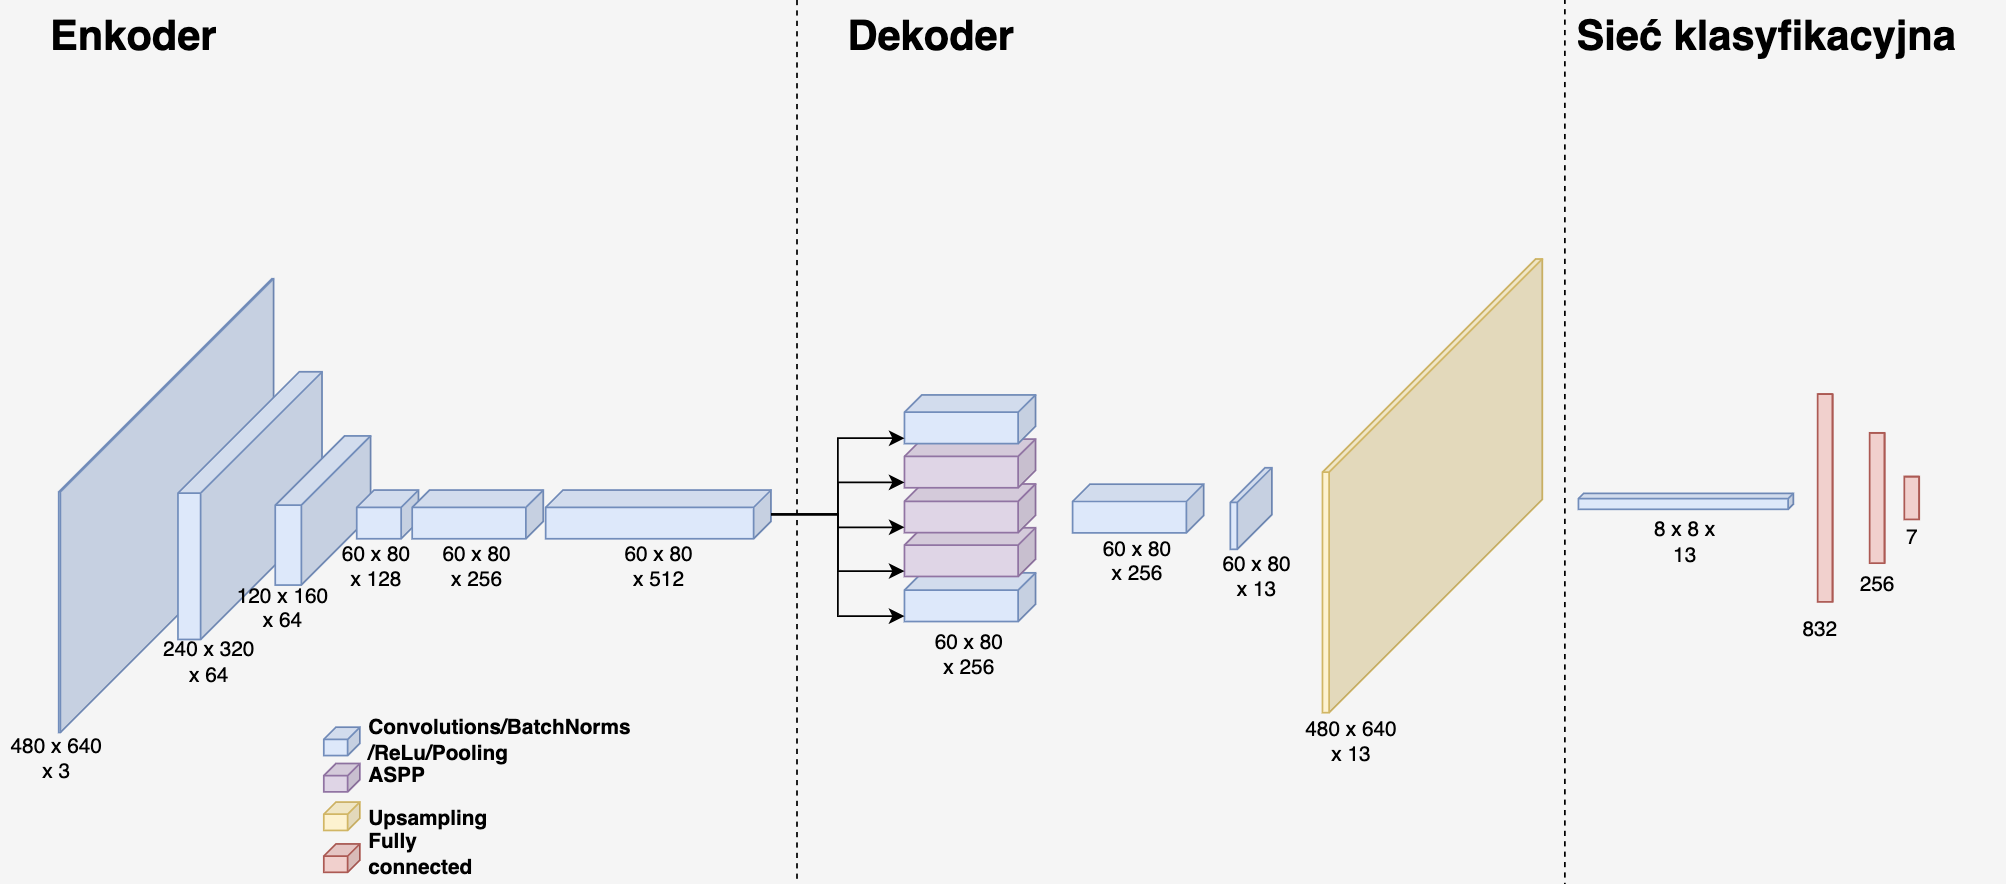
\includegraphics[width=\textwidth]{multitask-arch-seq-new.png}
    \caption{Architektura sieci szeregowej.}
    \label{fig:multitask-seq}
\end{figure}



\subsection{Zbiór  danych}
Dane są kluczową częścią głębokiego uczenia. Duży zbiór danych oznaczonych adnotacjami na poziomie pikseli jest potrzebny do wytrenowania wydajnego modelu segmentacji semantycznej. Typowe zestawy danych do segmentacji semantycznej to Cityscapes, PASCAL VOC i ADE20K. Podobnie w przypadku klasyfikacji sceny wymagany jest duży zbiór danych z odpowiednią informacją o etykiecie. Popularne zestawy danych do klasyfikacji scen obejmują NYUv2, SUN RGB-D, Matterport3D i ScanNet.
\subsubsection{Wybór zbioru danych}
Po prześledzeniu wielu zbiorów danych udało się sprostać wymaganiom pracy, uzyskując dwa podobne zbiory danych - \texttt{NYUv2} oraz \texttt{SUN RGBD}. Ostatecznie wybrano \texttt{NYUv2}. Trudno jednozczanie odpowiedzieć, który zbiór jest lepszy. Wykorzystano fakt cytowalności. Okazuje się, że \texttt{NYUv2} jest też chętniej cytowany niż \texttt{SUN RGBD} (rys. \ref{fig:sun-vs-nyu}), zatem to ten zbiór właśnie wybrano.

\begin{figure}[ht!]
    \centering
    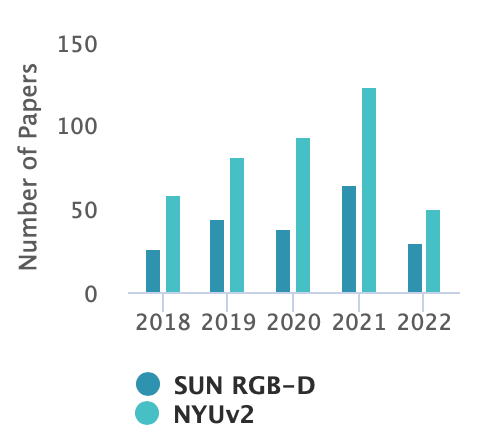
\includegraphics[width=0.5\textwidth]{img/stats-dataset.png}
    \caption[]{Szacowana liczba cytowań w latach 2018-2022 \href{https://paperswithcode.com/dataset/sun-rgb-d}{[paperswithcode.com]}}
    \label{fig:sun-vs-nyu}
\end{figure}
\subsection{Analiza zbioru danych}
Eksploracyjna analiza danych (ang. EDA) to proces eksploracji i zrozumienia cech zbioru danych przed zbudowaniem modelu. Jednym z głównych powodów, dla których proces ten jest ważny w wizji komputerowej to fakt, że może pomóc w identyfikacji problemów ze zbiorem danych, takich jak nieprawidłowe etykiety. Co więcej, może ono być również wykorzystane do identyfikacji skośnych rozkładów klas prowadzących do niesprawiedliwych prognoz. EDA może być również wykorzystana do określenia, które kroki przetwarzania wstępnego (ang. preprocessing), takie jak augmentacja, są niezbędne do poprawy wydajności modelu wizji komputerowej. Badając dane i rozumiejąc ich charakterystykę, możemy uzyskać głębsze ich zrozumienie i zidentyfikować wszelkie problemy, które należy rozwiązać przed zbudowaniem modelu.

EDA przeprowadzone na zbiorze NYUv2 dostarczyło wielu interesujących szczegółów. W zbiorze domyślnie znajduje się 795 przykładów trenujących oraz 654 przykładów testujących. Ze zbioru testowego wyodrębniono zbiór walidacyjny stanowiący 20\% zbioru testowego. Ponadto sprawdzono rozkład klas na przestrzeni całego zbioru danych.
W przypadku zadania segmentacji semantycznej do dyspozycji był wybór 894, 40 lub 13 klas przedmiotów. Im rozróżnialność była większa, tym większe okazywały się dysproporcje w rozkładzie. Histogramy dla 13 i 40 klas przedstawiono na rysunku \ref{fig:rozklad-segm}.
Podobna sytuacja miała miejsce dla zadania klasyfikacji z tą różnicą, iż scalania klas należało dokonać ręcznie. Taki krok był kluczowy, gdyż pierwotny rozkład był silnie zdominowany przez kilka klas.
Ostatecznie wybrano 13 klas dla klasyfikacji (rys. \ref{fig:7 klas dystrybucja}) oraz scalone 7 dla segmentacji (rys. \ref{fig:7 klas dystrybucja}).

\begin{figure}[ht!]
\centering
\begin{subfigure}[b]{0.49\textwidth}
\centering
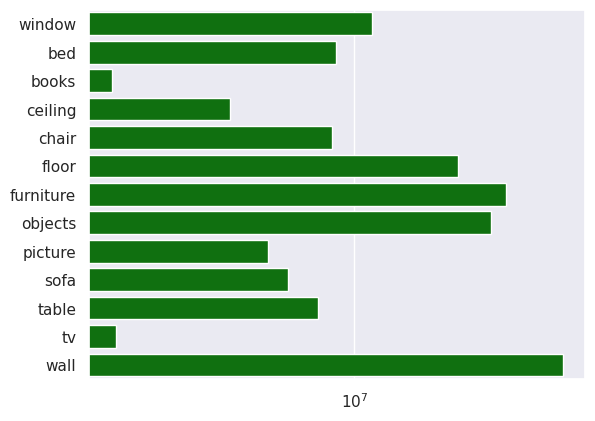
\includegraphics[width=\textwidth]{seg13.png}
\caption{Rozkład dla 13 klas.}
\label{fig:rozklad-13klas-seg}
\end{subfigure}
\hfill
\begin{subfigure}[b]{0.49\textwidth}
\centering
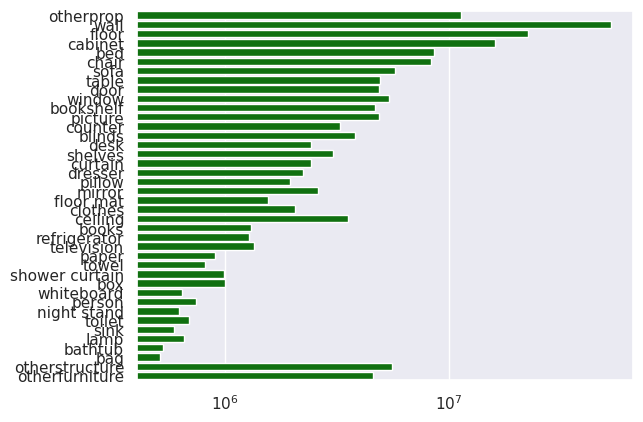
\includegraphics[width=\textwidth]{seg40.png}
\caption{Rozkład dla 40 klas.}
\label{fig:rozklad-40klas-seg}
\end{subfigure}
\caption[]{Porównanie rozkładu ilości pikseli dla zadania segmentacji semantycznej.}
\label{fig:rozklad-segm}
\end{figure}

\begin{figure}
\centering
\begin{subfigure}[b]{0.49\textwidth}
\centering
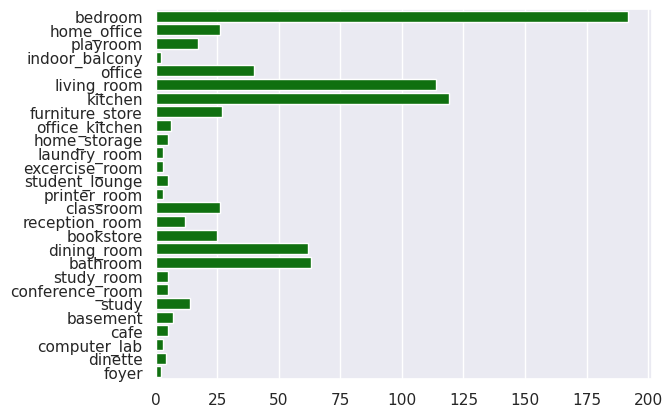
\includegraphics[width=\textwidth]{classification.png}
\caption{Oryginalny rozkład klas.}
\label{fig:27 klas dystrybucja}
\end{subfigure}
\hfill
\begin{subfigure}[b]{0.49\textwidth}
\centering
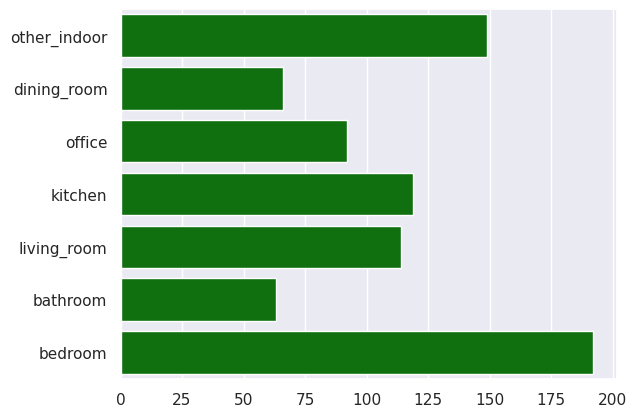
\includegraphics[width=\textwidth]{classification-merged.png}
\caption{Rozkład klas po scaleniu.}
\label{fig:7 klas dystrybucja}
\end{subfigure}
\caption[]{Porównanie rozkładu klas dla zadania klasyfikacji sceny.}
\end{figure}



% W celu łatwej oraz dokładniej ewaluaji 

% W celu lepsze ewaluacji uczenia wielozadaniowego zdecydowano uściślij wszystkie parametry sieci takie jak architekura jest ta sama zeby dało sie porownac nie

% nie ma sensu wszystkich scenariusz bo tak

% opisać że nie ma sensu porównywać 





























% Poza uczeniem łącznym zbadano też inne znane techniki uczenia jak finetuning.


% % * multitask Learning
% % * jednozadaniowe
% % * wielozadaniowe
% W celu realizacji zadania zdecydowano się na architekturę (najbliższą Y-Netu) o wspólnym enkoderze i o osobnych głowach, służących do egzekwowania konkretnych zadań (rys. \ref{fig:cep_arch}). Decyzja podyktowana była względnie prostą implementacją rozszerzenia wielu modeli segmentacji semantycznej o dodatkową głowę klasyfikacyjną. Co więcej stwierdzono, że ograniczenie się tylko do jednego backbone'u jest niesłychanie korzystne, gdyż znacząco ogranicza ilość parametrów sieci, co bezpośrednio przekłada się m.in. na czas inferencji. Należy zwrócić uwagę na fakt, iż właściwie zdecydowana większość parametrów znajduje się własnie w enkoderze.

% Mając na uwadze, że symultaniczne uczenie może negatywnie wpływać na jakość uczenia obu zadań, eksperymenty przeprowadzono etapowo. Pierwszym etapem było uczenie jednozadaniowe. Eksperymenty polegały na sprawdzeniu jakości segmentacji oraz klasyfikacji osobno. Wykorzystano do tego tę samą archtekturę, która używana była poźniej w drugim etapie. Mianowicie, mając dwie głowy każdorazowo zamrażano głowę nie biorącą udziału w uczeniu (rys. \ref{fig:arch-scene-seg}). Zapewnia to pewność posiadania tej samej architektury, a w szczególności rzetelne porównanie z etapem uczenia wielozadaniowego.

% Drugim etapem było przeprowadzenie eksperymentów w uczeniu wielozadaniowym (rys. \ref{fig:arch-full}). Funkcja celu zdefiniowana była jako suma wartości funkcji celów dla obu zadań. W wyniku progpagacji wstecznej wagi aktualizowane były zgodnie z zagregowaną stratą.

% Ostatecznie porównano jakość na przesztreni obu etapów.

% \begin{figure}[ht!]
%     \centering
%     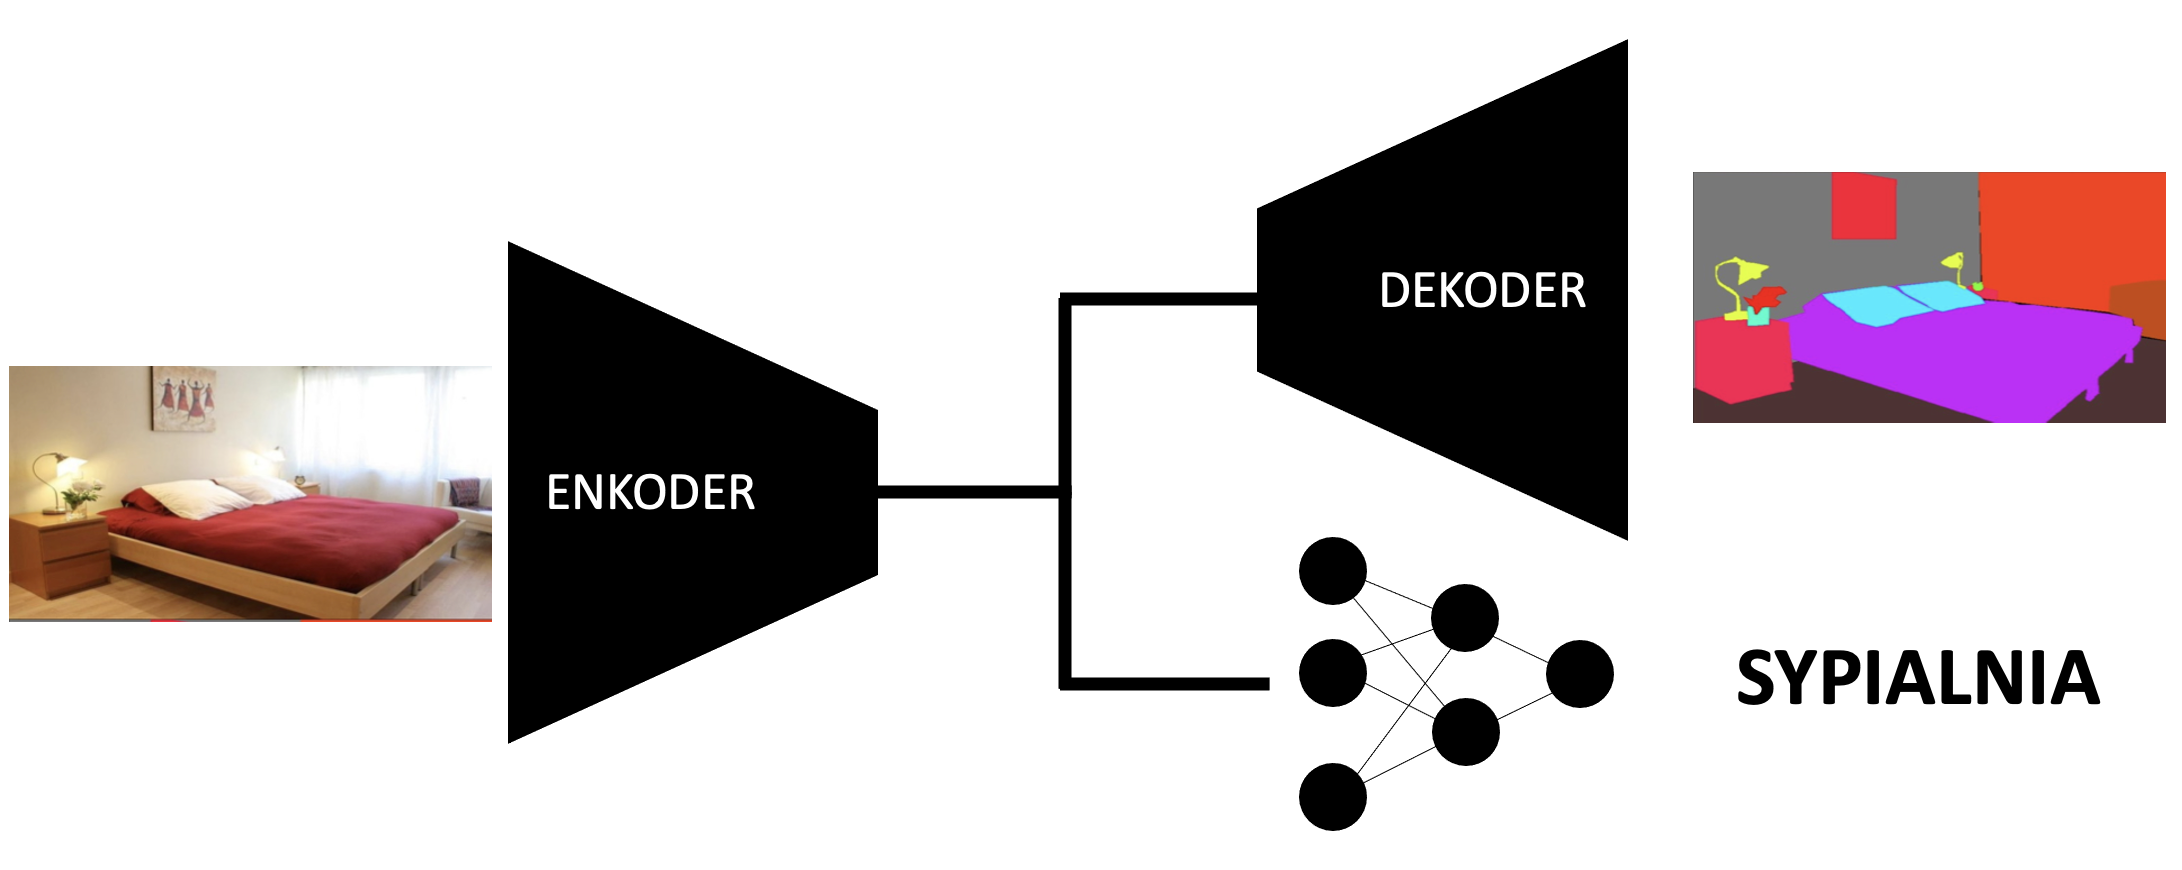
\includegraphics[width=0.75\textwidth]{cep_arch.png}
%     \caption{Architektura sieci zastosowana w pracy inżynierskiej.}
%     \label{fig:cep_arch}
% \end{figure}

% \begin{figure}[ht!]
%     \centering
%     \begin{subfigure}[b]{0.49\textwidth}
%         \centering
%         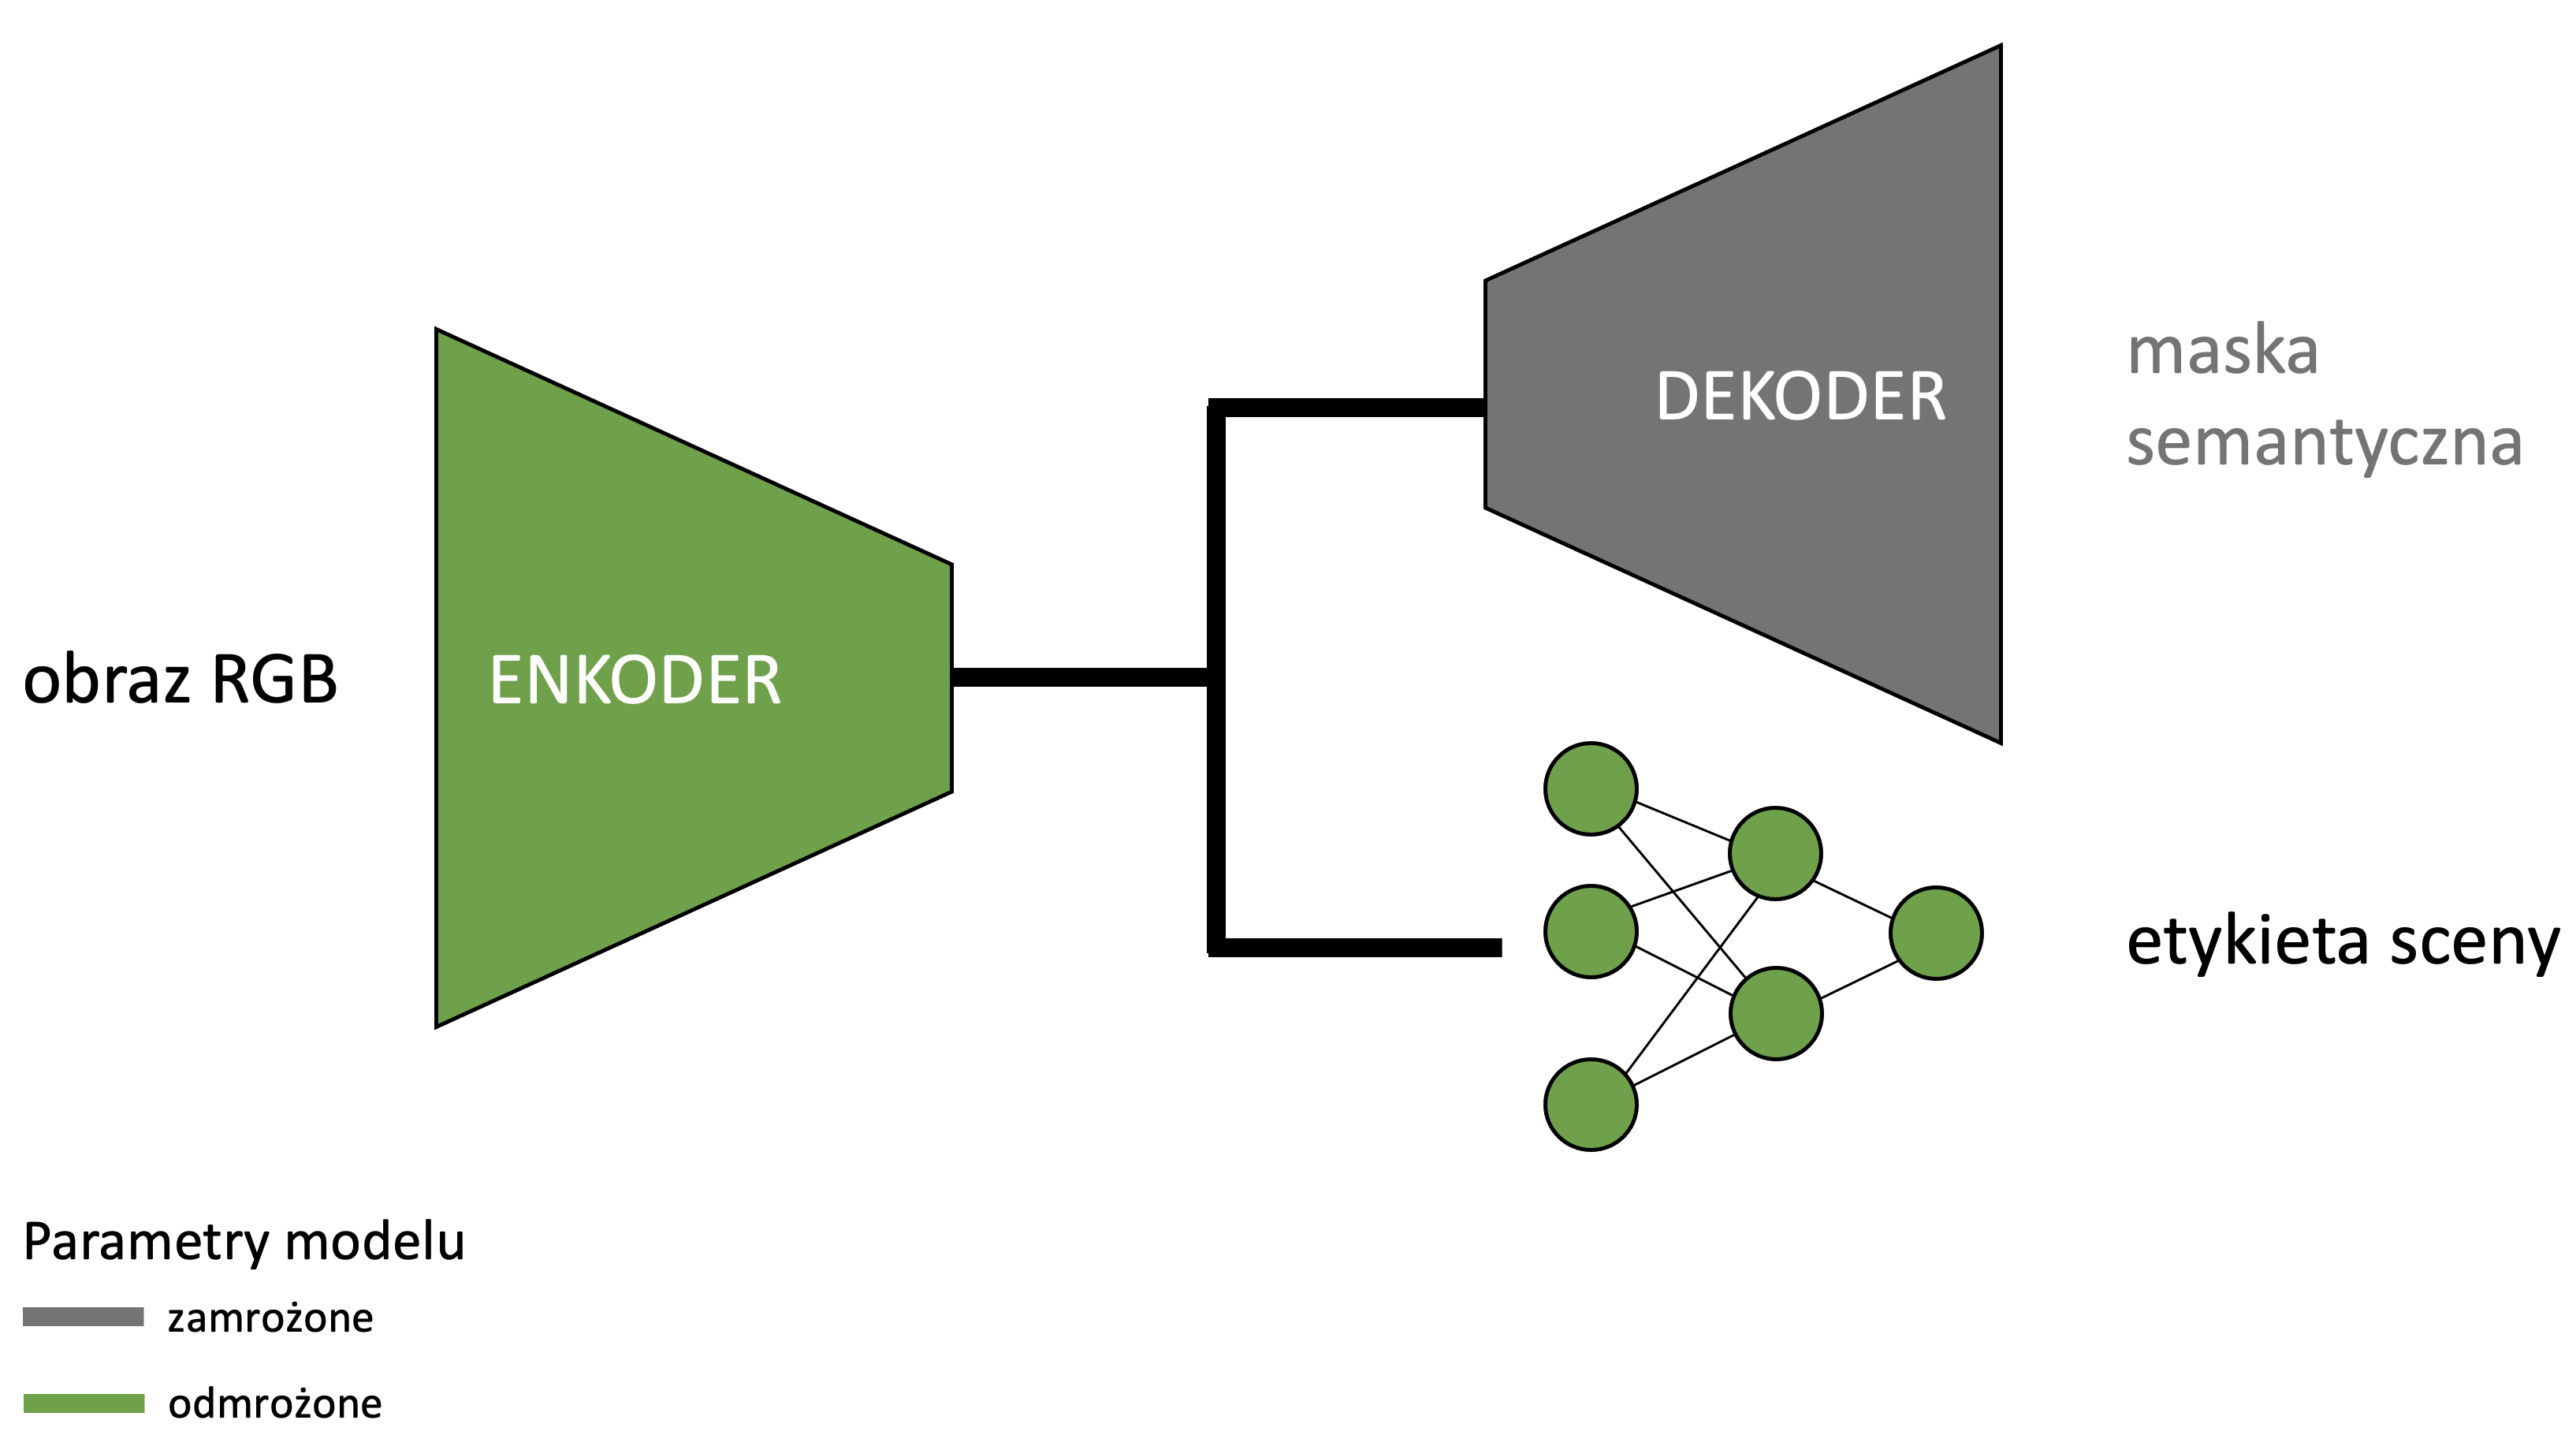
\includegraphics[width=\textwidth]{arch:scene.png}
%         \caption{Architektura sieci wyłącznie w zadaniu klasyfikacji.}
%     \end{subfigure}
%     \hfill
%     \begin{subfigure}[b]{0.49\textwidth}
%         \centering
%         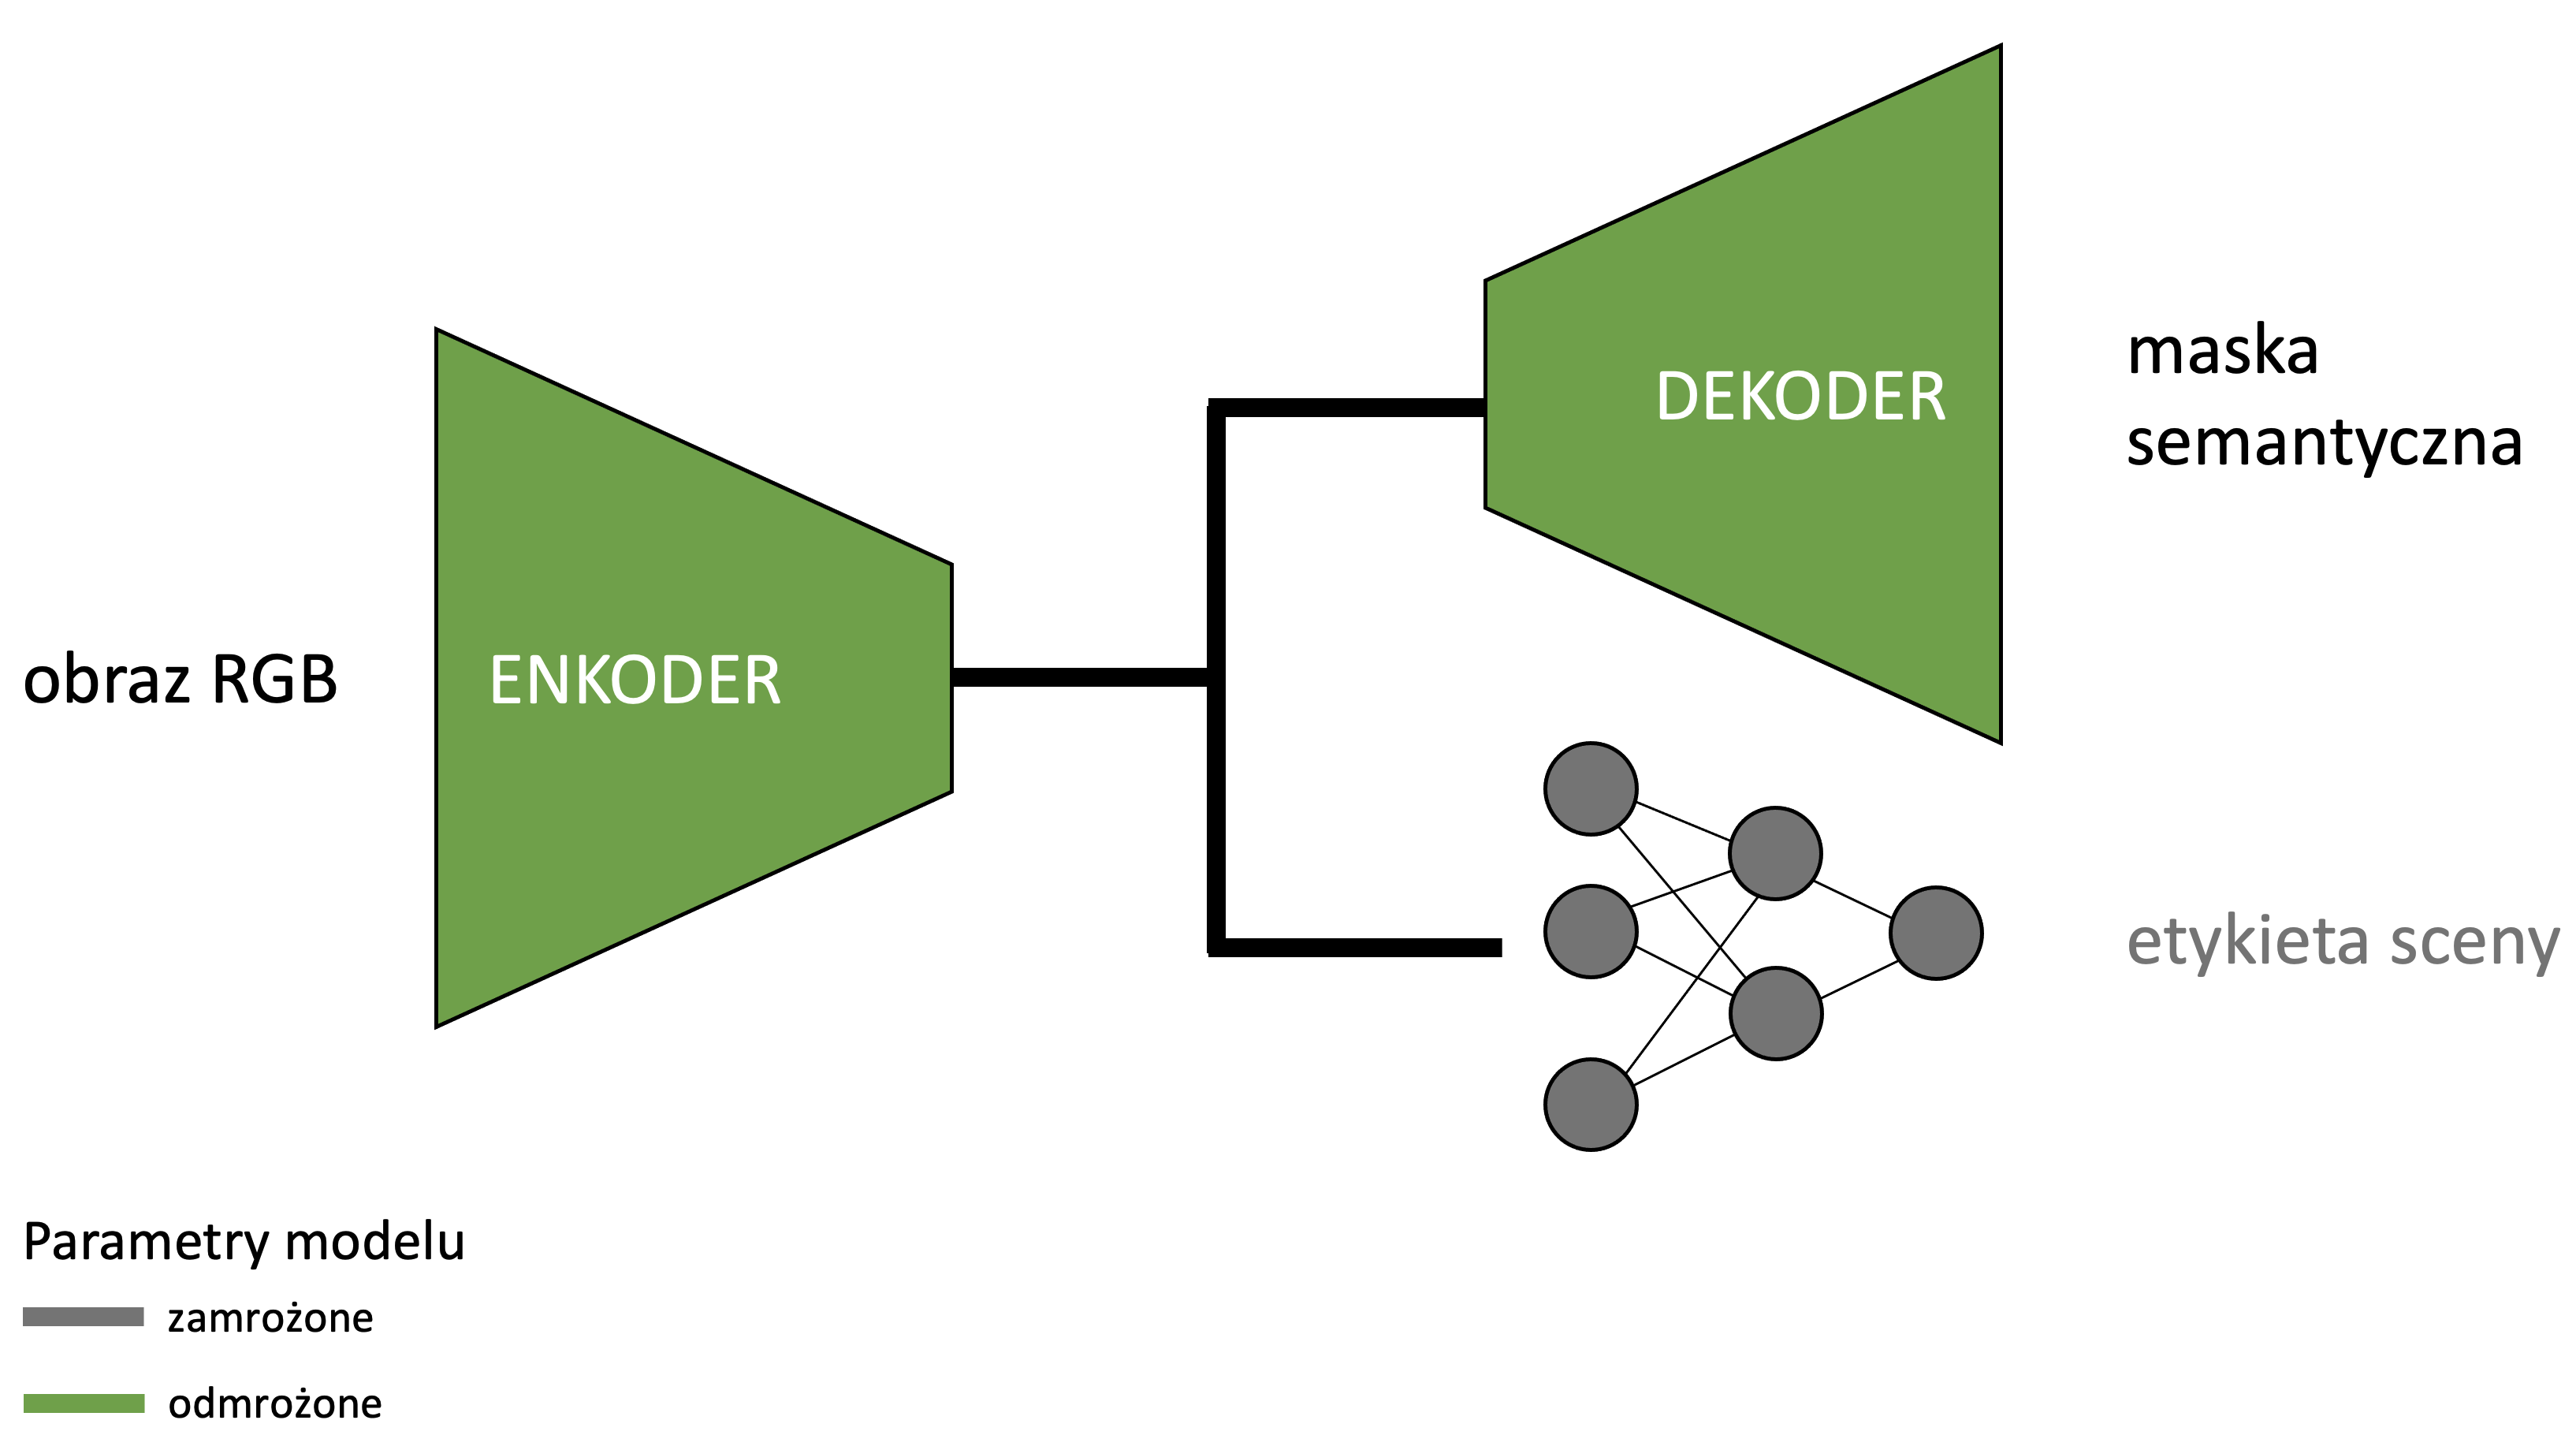
\includegraphics[width=\textwidth]{arch:seg.png}
%         \caption{Architektura sieci wyłącznie w zadaniu segmentacji semantycznej.}
%     \end{subfigure}
%     \caption[]{Podejście jednozadaniowe.}
%     \label{fig:arch-scene-seg}
% \end{figure}

% \begin{figure}[ht!]
%     \centering
%     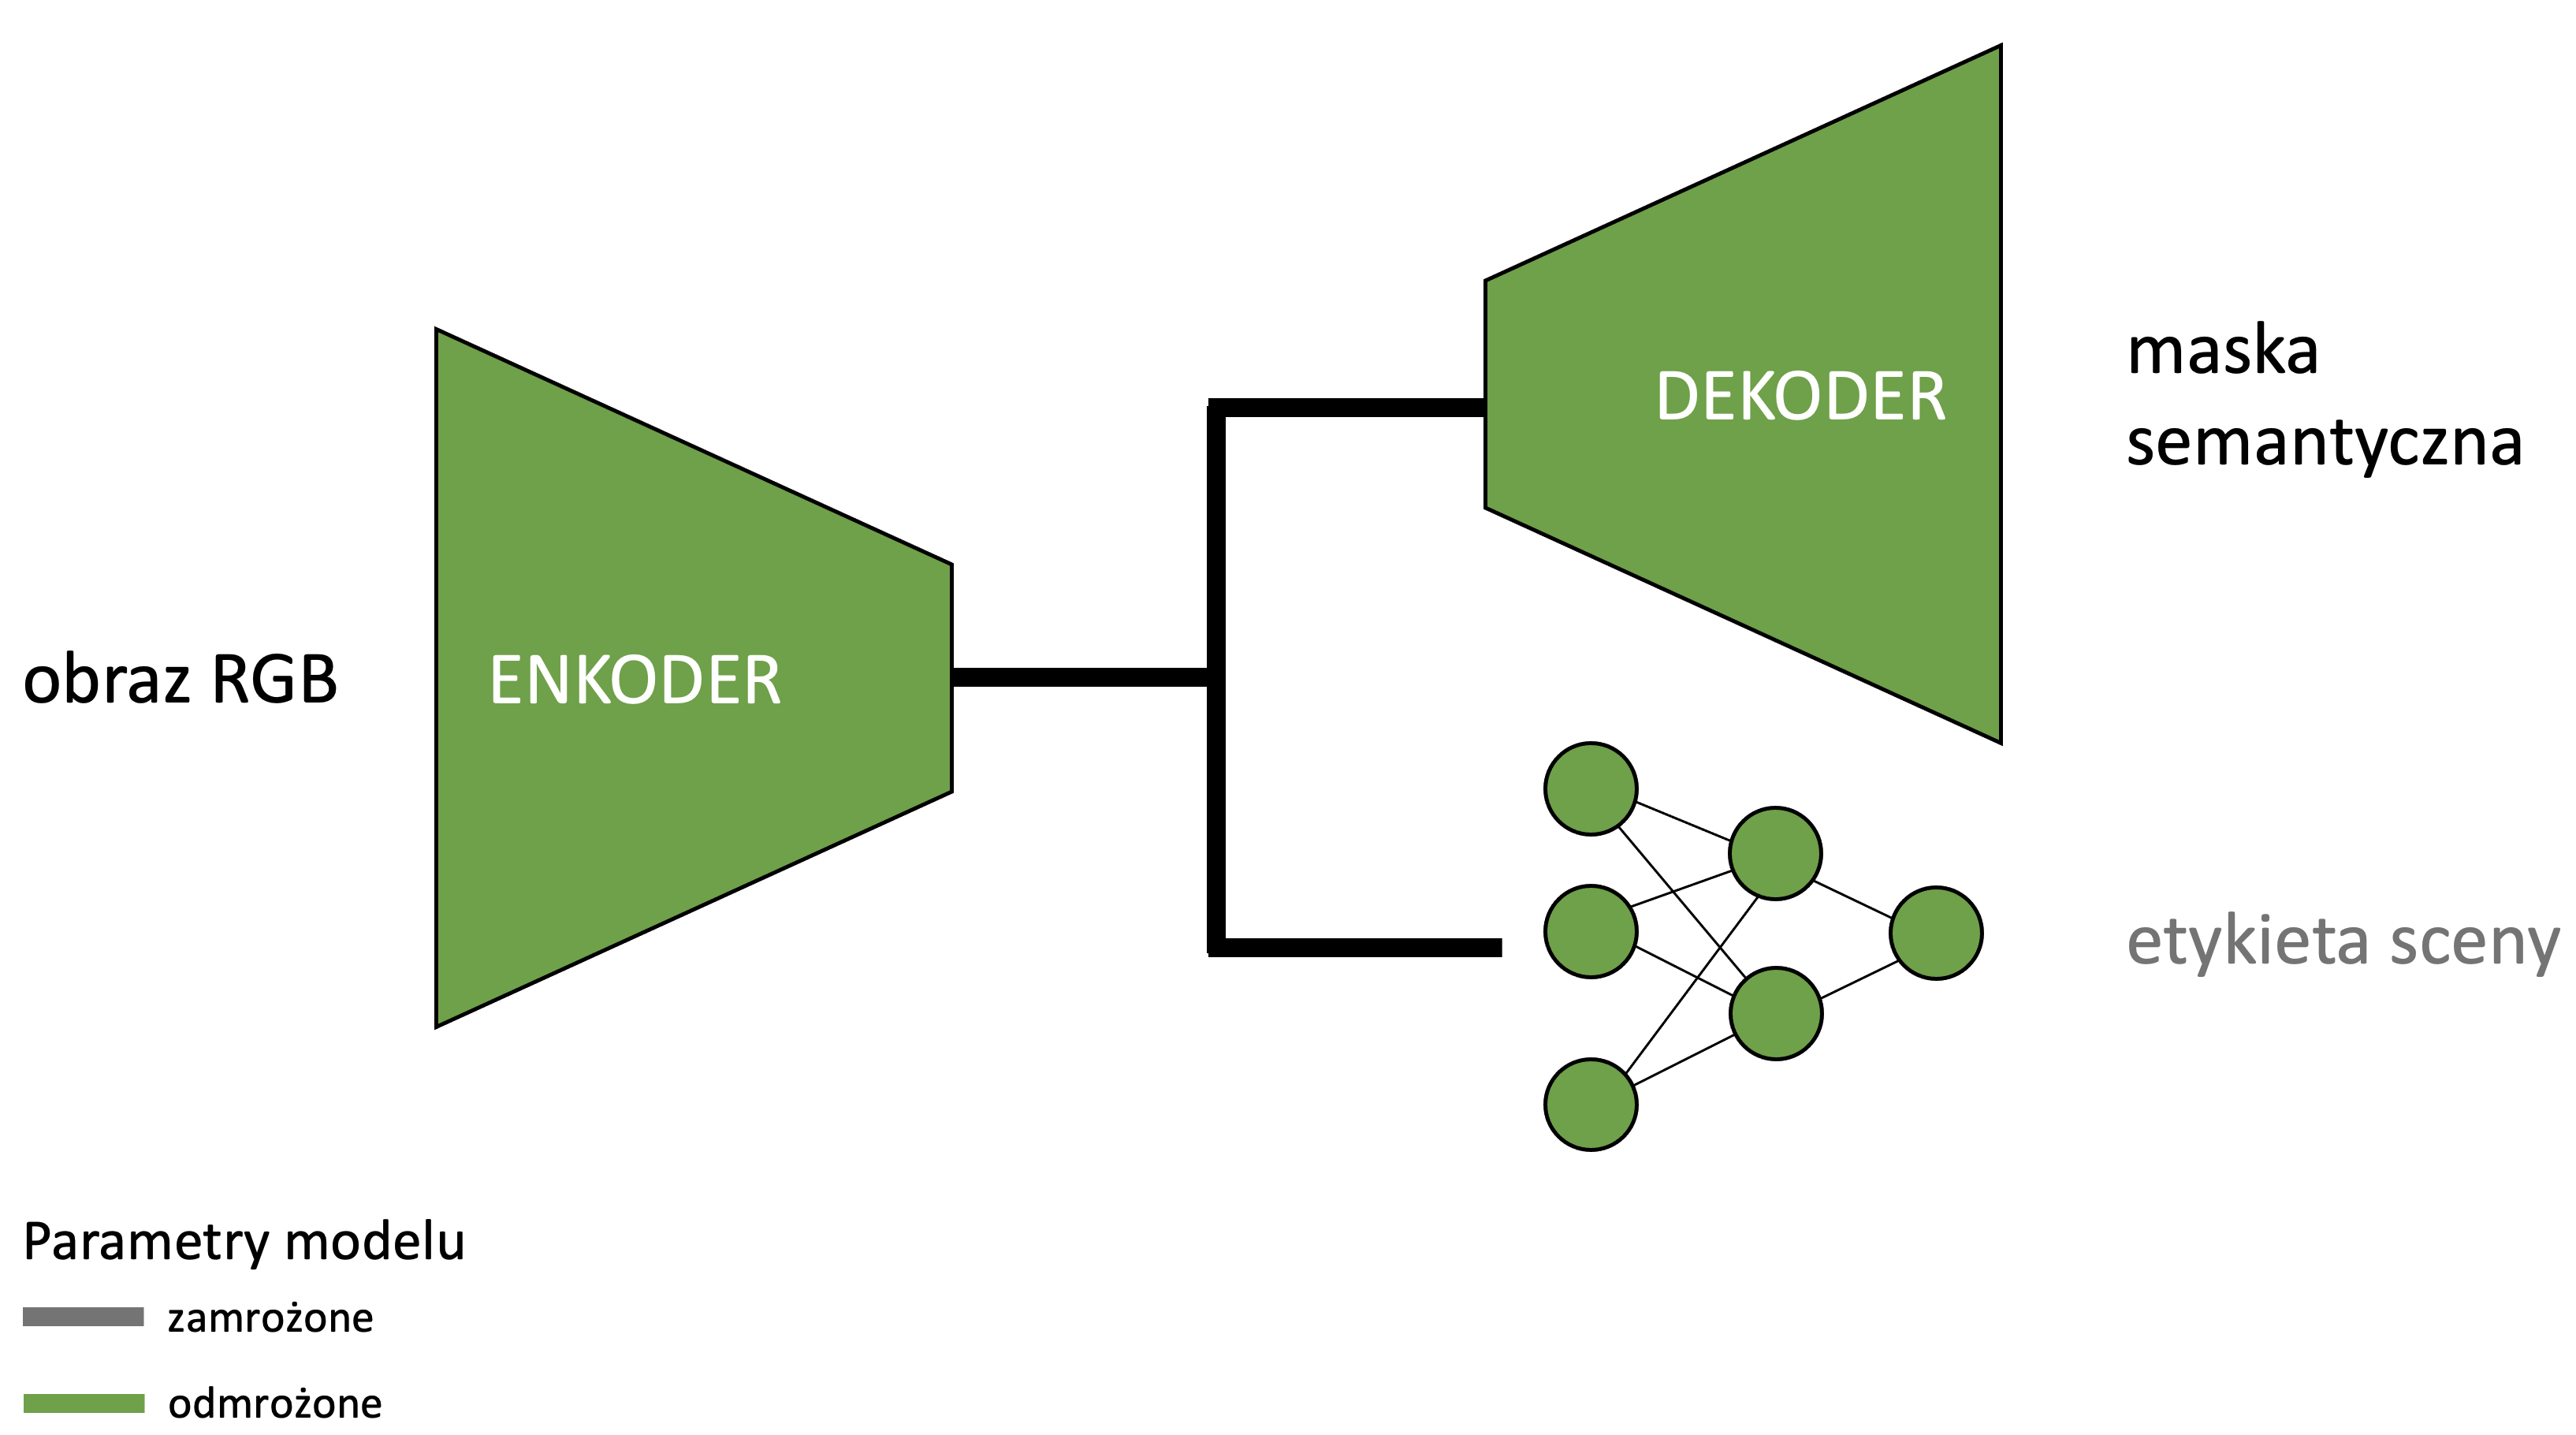
\includegraphics[width=0.75\textwidth]{arch:full.png}
%     \caption{Architektura sieci jako uczenie wielozadaniowego.}
%     \label{fig:arch-full}
% \end{figure}
\newpage % Rozdziały zaczynamy od nowej strony.
\section{Eksperymenty}
\subsection{Zbiór  danych}
Dane są kluczową częścią głębokiego uczenia. Duży zbiór danych oznaczonych adnotacjami na poziomie pikseli jest potrzebny do wytrenowania wydajnego modelu segmentacji semantycznej. Typowe zestawy danych do segmentacji semantycznej to Cityscapes, PASCAL VOC i ADE20K. Podobnie w przypadku klasyfikacji sceny wymagany jest duży zbiór danych z odpowiednią informacją o etykiecie. Popularne zestawy danych do klasyfikacji scen obejmują  NYUv2, SUN RGB-D, Matterport3D i ScanNet.



Zbiór danych powinien ściśle odpowiadać założeniom postawionym w pracy. Inferencja wymaga użycia kamery Kinect. Zatem zbiór danych powinien zawierać kategorie scen, segmentacje obrazów oraz najlepiej być ujętym przez kamerę Kinect wersji pierwszej.

Po prześledzeniu wielu zbiorów danych udało się sprostać powyższym wymaganiom, uzyskując dwa podobne zbiory danych - \texttt{NYUv2} oraz \texttt{SUN RGBD}. Ostatecznie wybrano \texttt{NYUv2} z uwagi, że zbiór ten został zawiera zdjecia
pomieszczeń, w które nie są posprzątane. Fakt ten uznano, za ważny, iż uważano, że będzie przekładał się na lepsze rezultaty w naturalnych warunkach. Co więcej \texttt{NYUv2} jest też chętniej cytowany niż \texttt{SUN RGBD} (rys. \ref{fig:sun-vs-nyu}).

\begin{figure}[ht!]
    \centering
    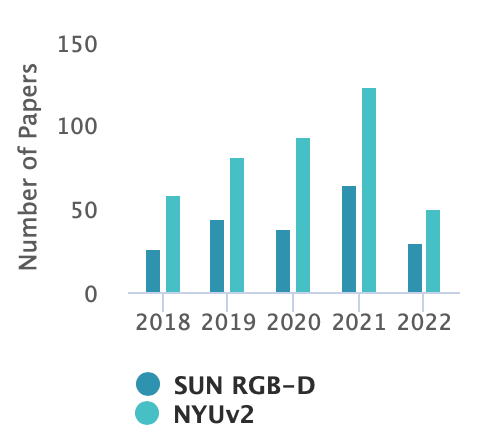
\includegraphics[width=0.5\textwidth]{img/stats-dataset.png}
    \caption[]{Szacowana liczba cytowań w latach 2018-2022 \href{https://paperswithcode.com/dataset/sun-rgb-d}{[paperswithcode.com]}}
    \label{fig:sun-vs-nyu}
\end{figure}

\subsection{Analiza zbioru danych}
Eksploracyjna analiza danych (ang. EDA) to proces eksploracji i zrozumienia cech zbioru danych przed zbudowaniem modelu. Omówione zostanie znaczenie EDA w głębokim uczeniu oraz możliwości wykorzystania do poprawy wydajności i interpretowalności modeli głębokiego uczenia.

Jakość danych

Jednym z głównych powodów, dla których EDA jest ważne w wizji komputerowej, jest to, że może pomóc w identyfikacji problemów ze zbiorem danych, takich jak brakujące wartości, wartości odstające lub nieprawidłowe etykiety, które mogą wpłynąć na wydajność modelu wizji komputerowej. Przeprowadzając EDA, możemy uzyskać głębsze zrozumienie danych i zidentyfikować wszelkie problemy, które należy rozwiązać przed zbudowaniem modelu.

Wstępne przetwarzanie danych

EDA może być również wykorzystana do określenia, które kroki przetwarzania wstępnego (ang. preprocessing), takie jak augmentacja, są niezbędne do poprawy wydajności modelu wizji komputerowej. Badając dane i rozumiejąc ich charakterystykę, jesteśmy w stanie lepiej dostosować różne techniki wstępnego przetwarzania danych.

Identyfikacja tendencyjności

EDA może być również wykorzystana do identyfikacji potencjalnych błędów w zbiorze danych, takich jak skośne rozkłady klas, które mogą wpływać na wydajność modelu widzenia komputerowego i prowadzić do niesprawiedliwych prognoz. Przeprowadzając EDA, możemy zidentyfikować wszelkie uprzedzenia w danych i podjąć kroki w celu ich rozwiązania przed zbudowaniem modelu.

% Wnioski

% Podsumowując, prowadzenie EDA jest ważne w wizji komputerowej, ponieważ może pomóc poprawić wydajność modelu, zwiększyć jego interpretowalność i zapewnić, że model jest sprawiedliwy i bezstronny. EDA może być wykorzystana do identyfikacji problemów ze zbiorem danych, wyboru odpowiednich cech, wstępnego przetwarzania danych, zrozumienia zachowania modelu i zidentyfikowania potencjalnych stronniczości. Przeprowadzając EDA, możemy uzyskać głębsze zrozumienie danych oraz poprawić wydajność i interpretowalność modelu widzenia komputerowego.

EDA przeprowadzone na zbiorze NYUv2 dostarczyło wielu interesujących szczegółów. W zbiorze domyślnie znajduje się 795 przykładów trenujących oraz 654 przykładów testujących. Ze zbioru testowego wyodrębniono zbiór walidacyjny stanowiący 20\% zbioru testowego. Ponadto sprawdzono rozkład klas na przesztrzeni całego zbioru danych.
W przypadku zadania segmentacji semantycznej do dyspozycji był wybór 894, 40 lub 13 klas przedmiotów. Im rozróżnialność była większa tym większe okazywały się dysproporcje w rozkładzie. Histogramy dla 13 i 40 klas przedstawiono na rysunku \ref{fig:rozklad-segm}.
Podobna sytuacja miała miejsce dla zadania klasyfikacji z tą różnicą, iż scalania klas należało dokonać ręcznie. Taki krok był kluczowy, gdyż pierwotny rozkład był silnie zdominowany przez kilka klas.
Ostatecznie wybrano 13 klas dla klasyfikacji (rys. \ref{fig:7 klas dystrybucja}) oraz scalone 7 dla segmentacji (rys. \ref{fig:7 klas dystrybucja}).
\begin{figure}[ht!]
    \centering
    \begin{subfigure}[b]{0.49\textwidth}
        \centering
        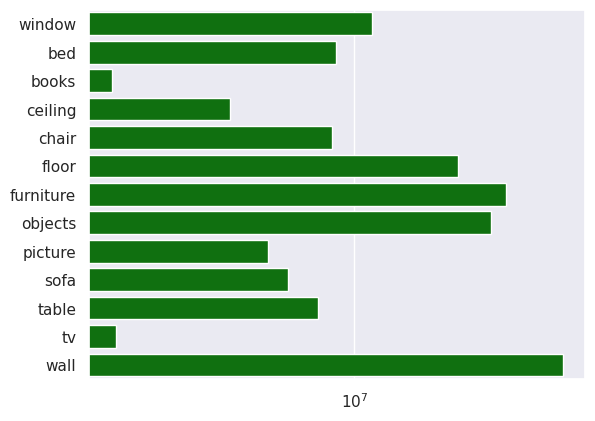
\includegraphics[width=\textwidth]{seg13.png}
        \caption{Rozkład dla 13 klas.}
        \label{fig:rozklad-13klas-seg}
    \end{subfigure}
    \hfill
    \begin{subfigure}[b]{0.49\textwidth}
        \centering
        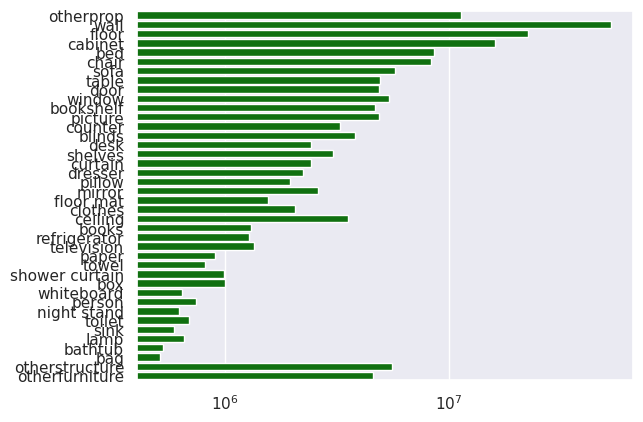
\includegraphics[width=\textwidth]{seg40.png}
        \caption{Rozkład dla 40 klas.}
        \label{fig:rozklad-40klas-seg}
    \end{subfigure}
    \caption[]{Porównanie rozkładu ilości pixeli dla zadania segmentacji semantycznej.}
    \label{fig:rozklad-segm}
\end{figure}
\begin{figure}
    \centering
    \begin{subfigure}[b]{0.49\textwidth}
        \centering
        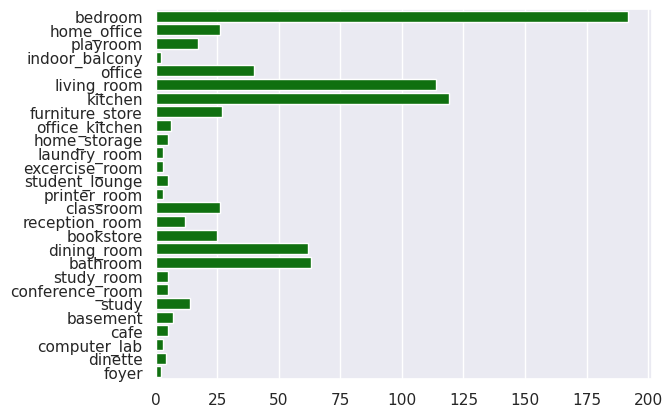
\includegraphics[width=\textwidth]{classification.png}
        \caption{Oryginalny rozkład klas.}
        \label{fig:27 klas dystrybucja}
    \end{subfigure}
    \hfill
    \begin{subfigure}[b]{0.49\textwidth}
        \centering
        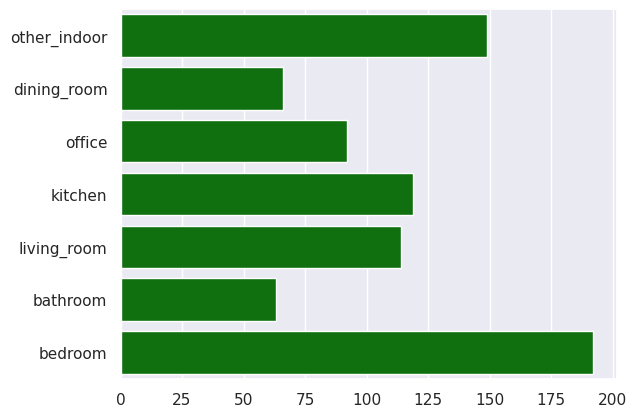
\includegraphics[width=\textwidth]{classification-merged.png}
        \caption{Rozkład klas po scaleniu.}
        \label{fig:7 klas dystrybucja}
    \end{subfigure}
    \caption[]{Porównanie rozkładu klas dla zadania klasyfikacji sceny.}
\end{figure}

% * wykorzystanie TU NICR
% * Wersje segmentacji: 13, 40 i 8xx klasowa
% * ile obrazków w jakich zbiorach.
% * wstawić przykładowe obrazki z datasetu
% * Konkatenacja dla klas dla klasyfikacji - dlaczego?
% * EDA - histogramy klas

\subsection{Opis eksperymentów}
\noindent
Przygotowanie danych

Obrazy RGB zostały poddane normalizacji ze średnią (0.485, 0.456, 0.406) oraz odchyleniem standardowym (0.229, 0.224, 0.225), która odpowiada parametrom rozkładu normlanego na zbiorze ImageNet. Baza ImageNet służyła do wytrenowania enkodera, a więc pierwszej części modelu.

Istnieje kilka różnych technik normalizacji, które mogą być stosowane w problemach z widzeniem komputerowym, takich jak normalizacja min-max i normalizacja rozkładem normalnym.  W pracy ,,Normalization Techniques in Training DNNs:
Methodology, Analysis and Application'' Lei et. al. \cite{huang2020normalization}, autorzy udowadjniają, że normalizacja stabilizuje i przyśpiesza trening oraz prawdopodobnie prowadzi do
do poprawy generalizacji. 

Normalizacja jest ważnym krokiem przetwarzania wstępnego w problemach widzenia komputerowego, ponieważ może pomóc w poprawieniu wydajności modelu. Normalizacja odnosi się do procesu skalowania danych wejściowych tak, aby miały w przybliżeniu średnią 0 i odchylenie standardowe 1. Pomaga to zapewnić, że dane wejściowe są w spójnym zakresie i mają podobny rozkład, co może poprawić model.
\noindent
Model

Jako  model użyto DeepLabv3, który rozszerzono o dodatkową głowę klasyfikacyjną. Umieszczono ją naturalnie zaraz za enkoderem, a przed dekoderem. Głowa klasyfikacyjna przedstawia się jako jako sieć w pełni połączona (FC) z dwiema warstwami.  

TO TRZEBA ZWIUZALIZOWAĆ!
\begin{addmargin}[6mm]{0mm}
    \begin{lstlisting}[
        language=Python,
        numbers=left,
        firstnumber=1,
        caption={Struktura głowy klasyfikacyjnej},
        aboveskip=0pt
    ]
    nn.AdaptiveAvgPool2d((1, 1)),
    nn.Flatten(),
    nn.BatchNorm1d(num_filters),
    nn.Dropout(p=0.25),
    nn.Linear(num_filters, out_features=256, bias=False),
    nn.ReLU(inplace=True),
    nn.BatchNorm1d(256),
    nn.Dropout(p=0.25),
    nn.Linear(in_features=256, out_features=scene_classes, bias=False),
    nn.Softmax(dim=1),
    \end{lstlisting}
    \end{addmargin}

\noindent
Funkcja straty

W obu przypadkach jako funkcję straty wykorzystano ważoną entropię skrośną. Wagi odzwierciedłały odwrotność liczności w zbiorze. Dla klasyfikacji liczona była ilość klas, natomiast dla segmentacji ilość pixeli.

\noindent
Uczenie

Uczenie odbywało się co najwyżej 50 epok aż do ustalenia się straty na zbiorze walidacyjnym. Krok uczenia był zmienny zgodnie z polityką One Cycle (rys.\ref{fig:one-cycle-policy}).


\begin{figure}[ht!]
    \centering
    \begin{subfigure}[b]{0.32\textwidth}
        \centering
        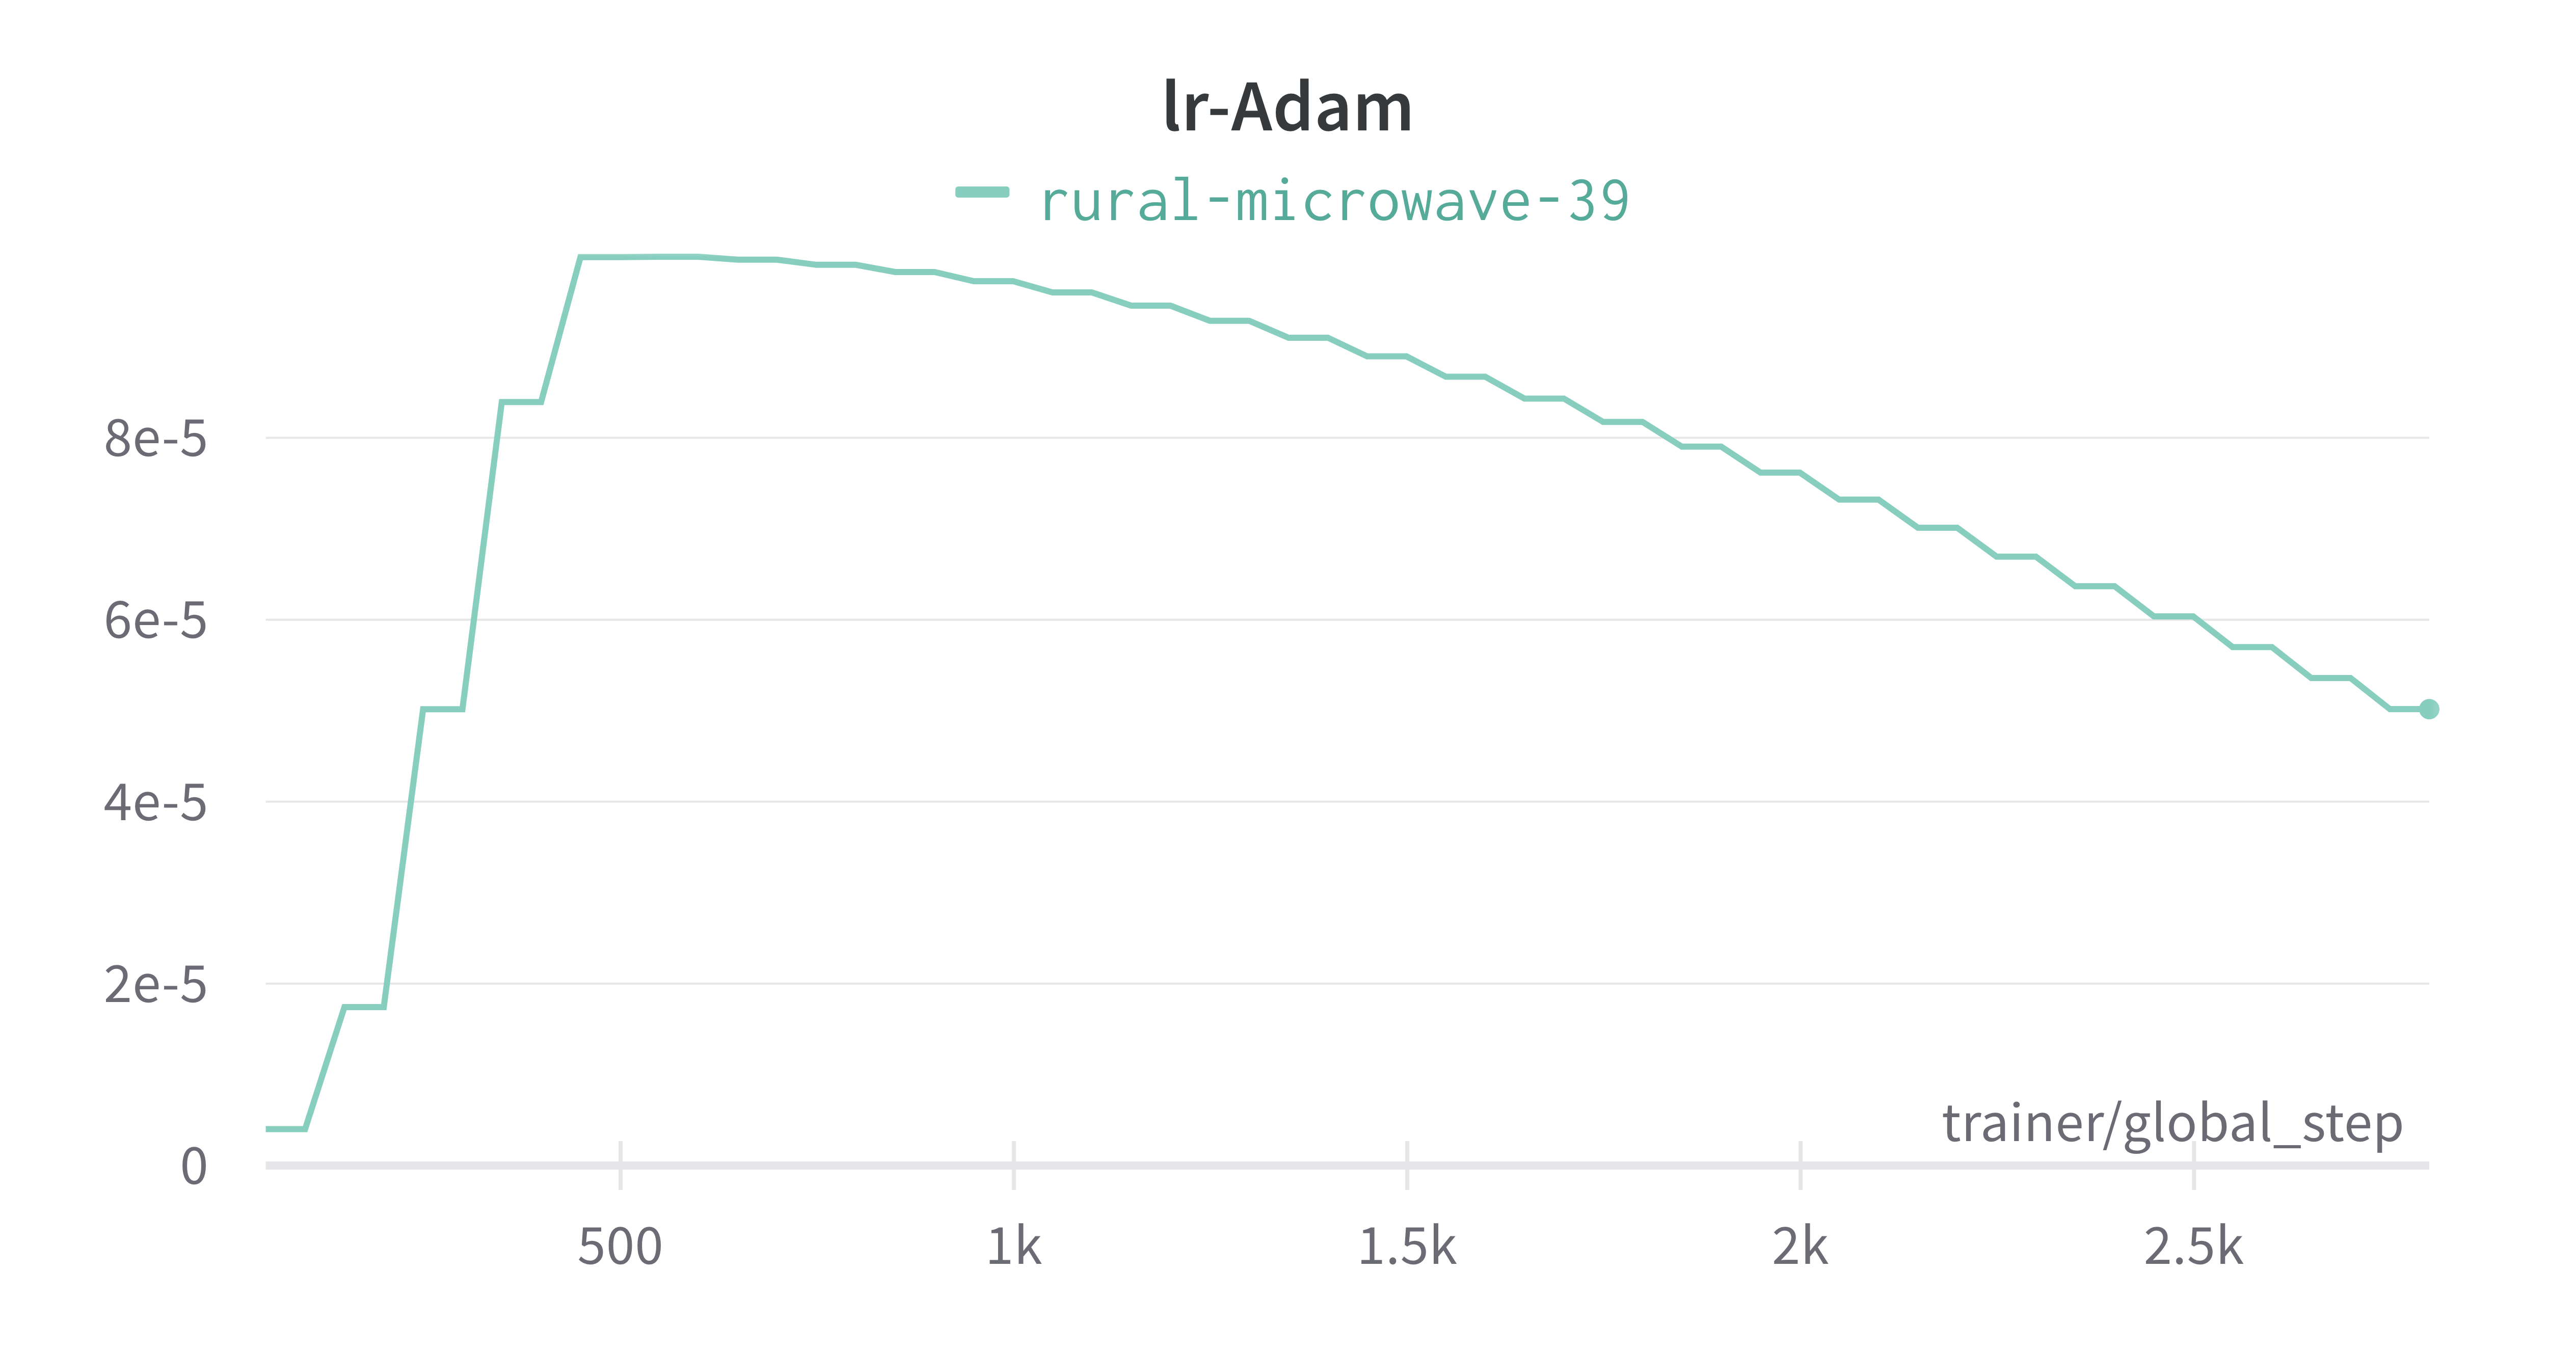
\includegraphics[width=\textwidth]{seg-lr.png}
        \caption{Segmentacja semantyczna.}
        % \label{fig:rozklad-13klas-seg}
    \end{subfigure}
    \hfill
    \begin{subfigure}[b]{0.32\textwidth}
        \centering
        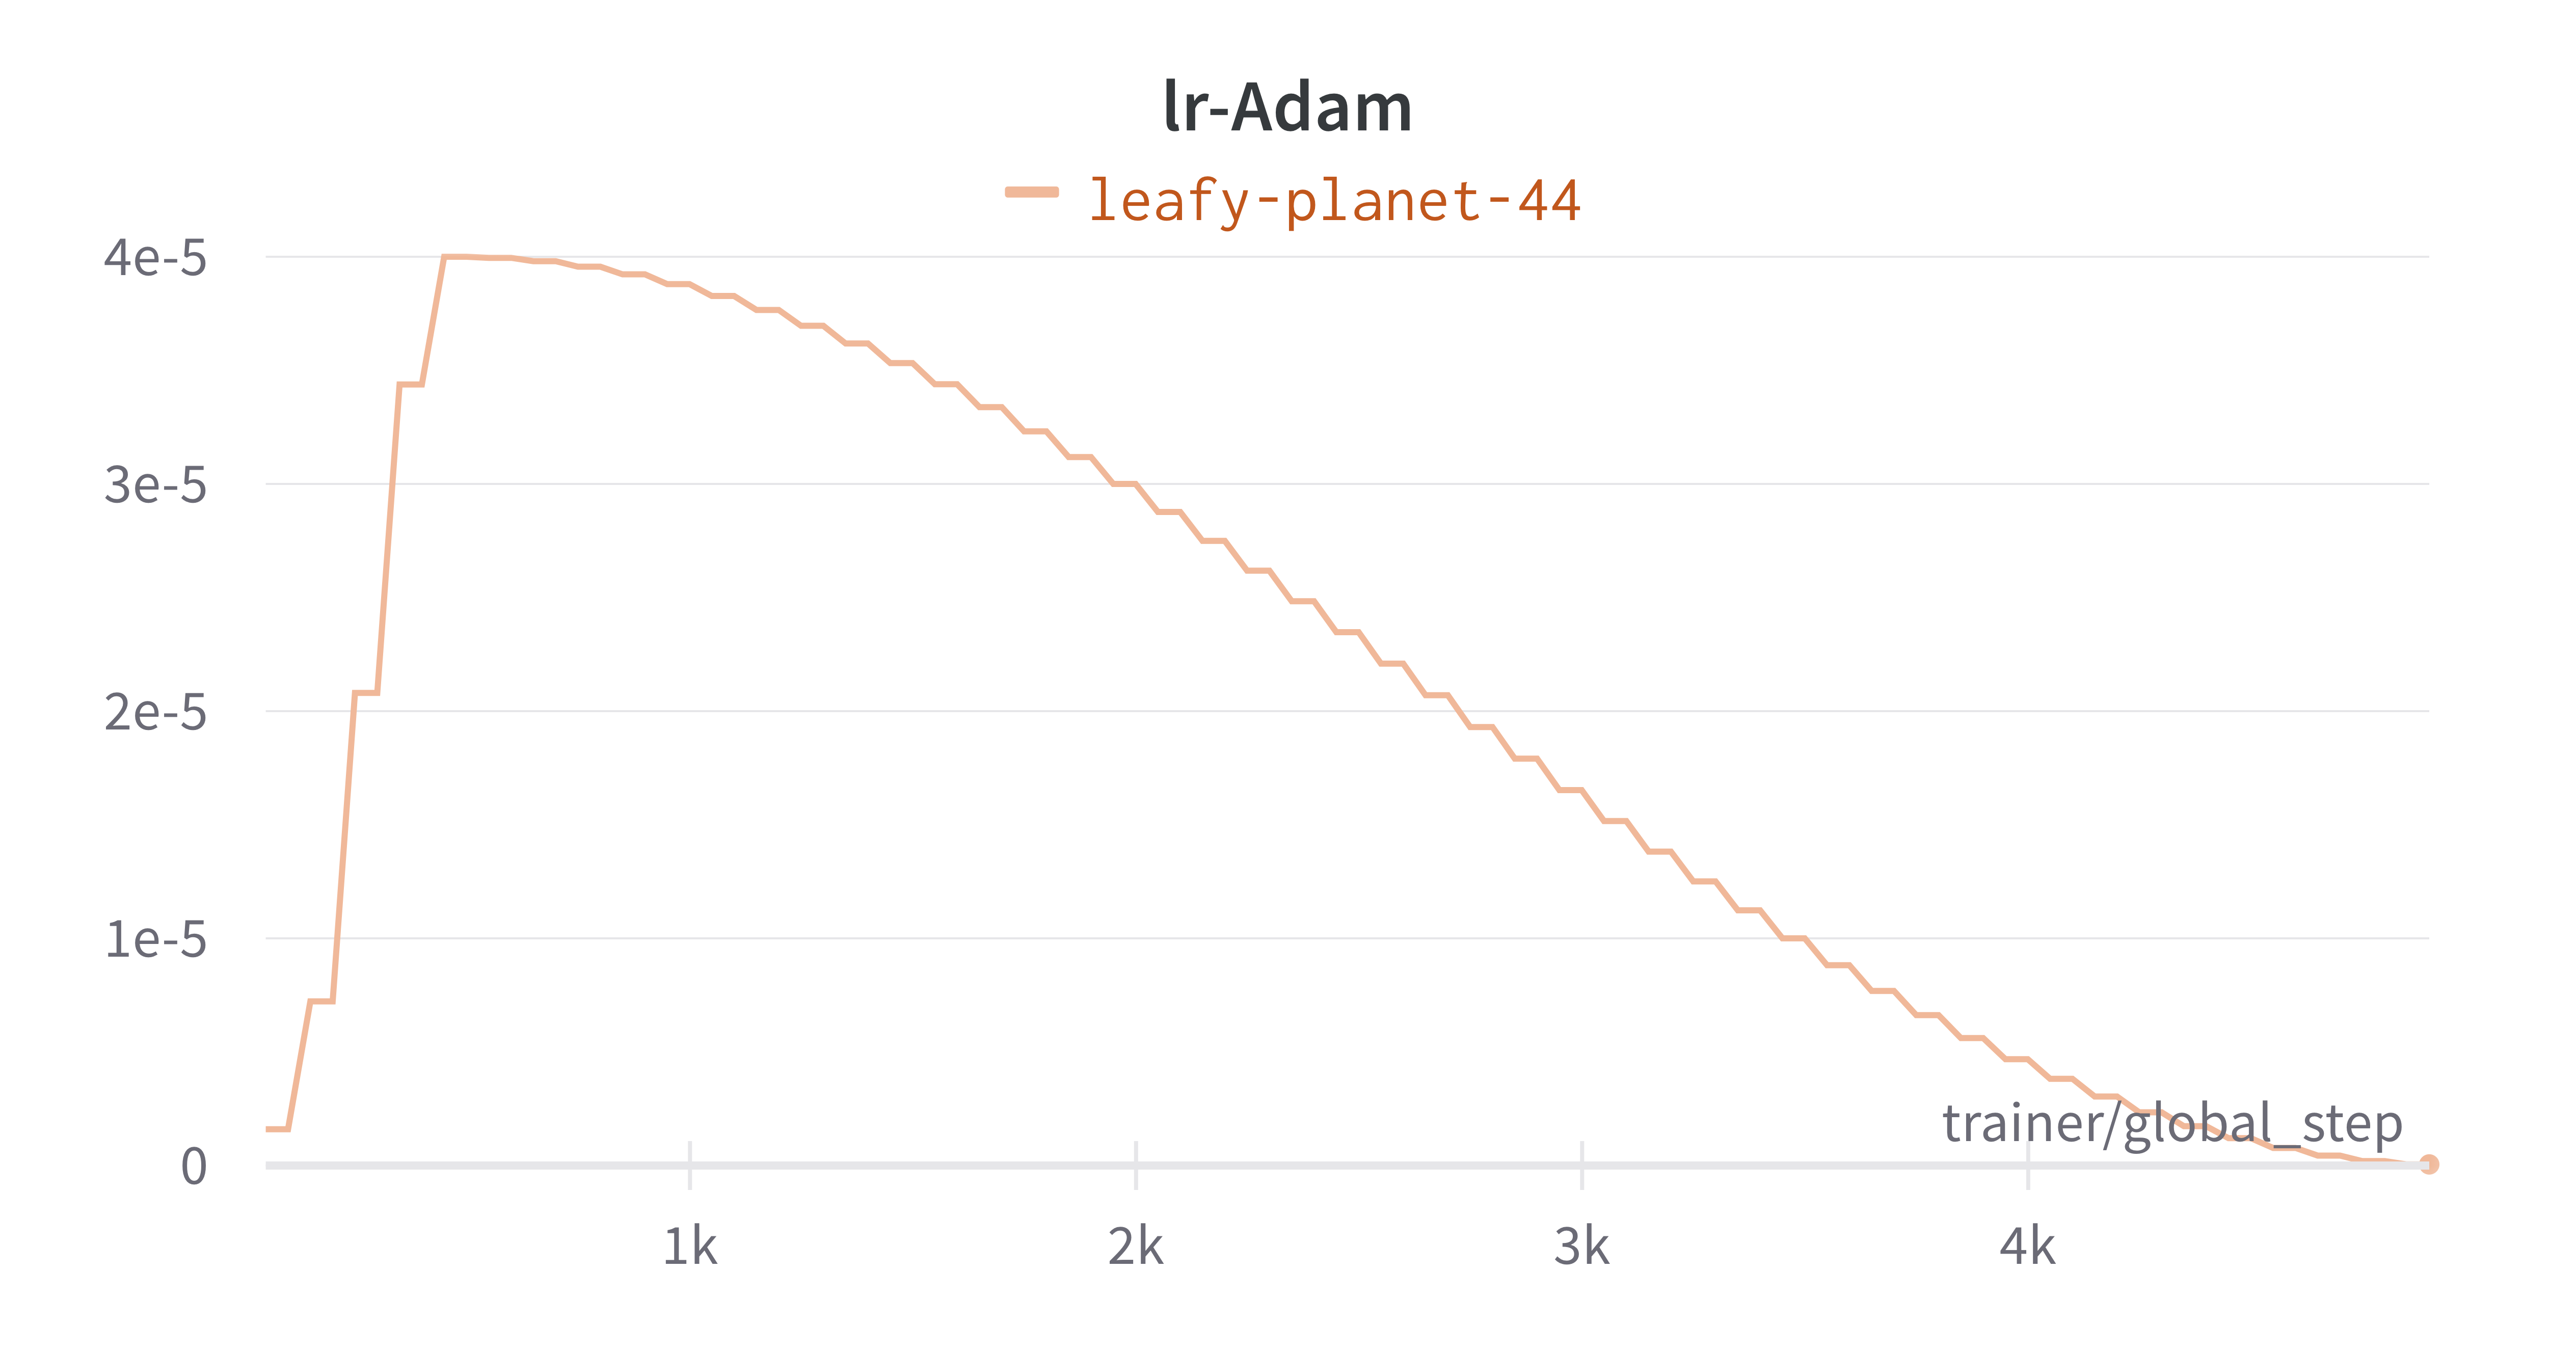
\includegraphics[width=\textwidth]{class-lr.png}
        \caption{Klasyfikacja sceny.}
        % \label{fig:rozklad-40klas-seg}
    \end{subfigure}
    \hfill
    \begin{subfigure}[b]{0.32\textwidth}
        \centering
        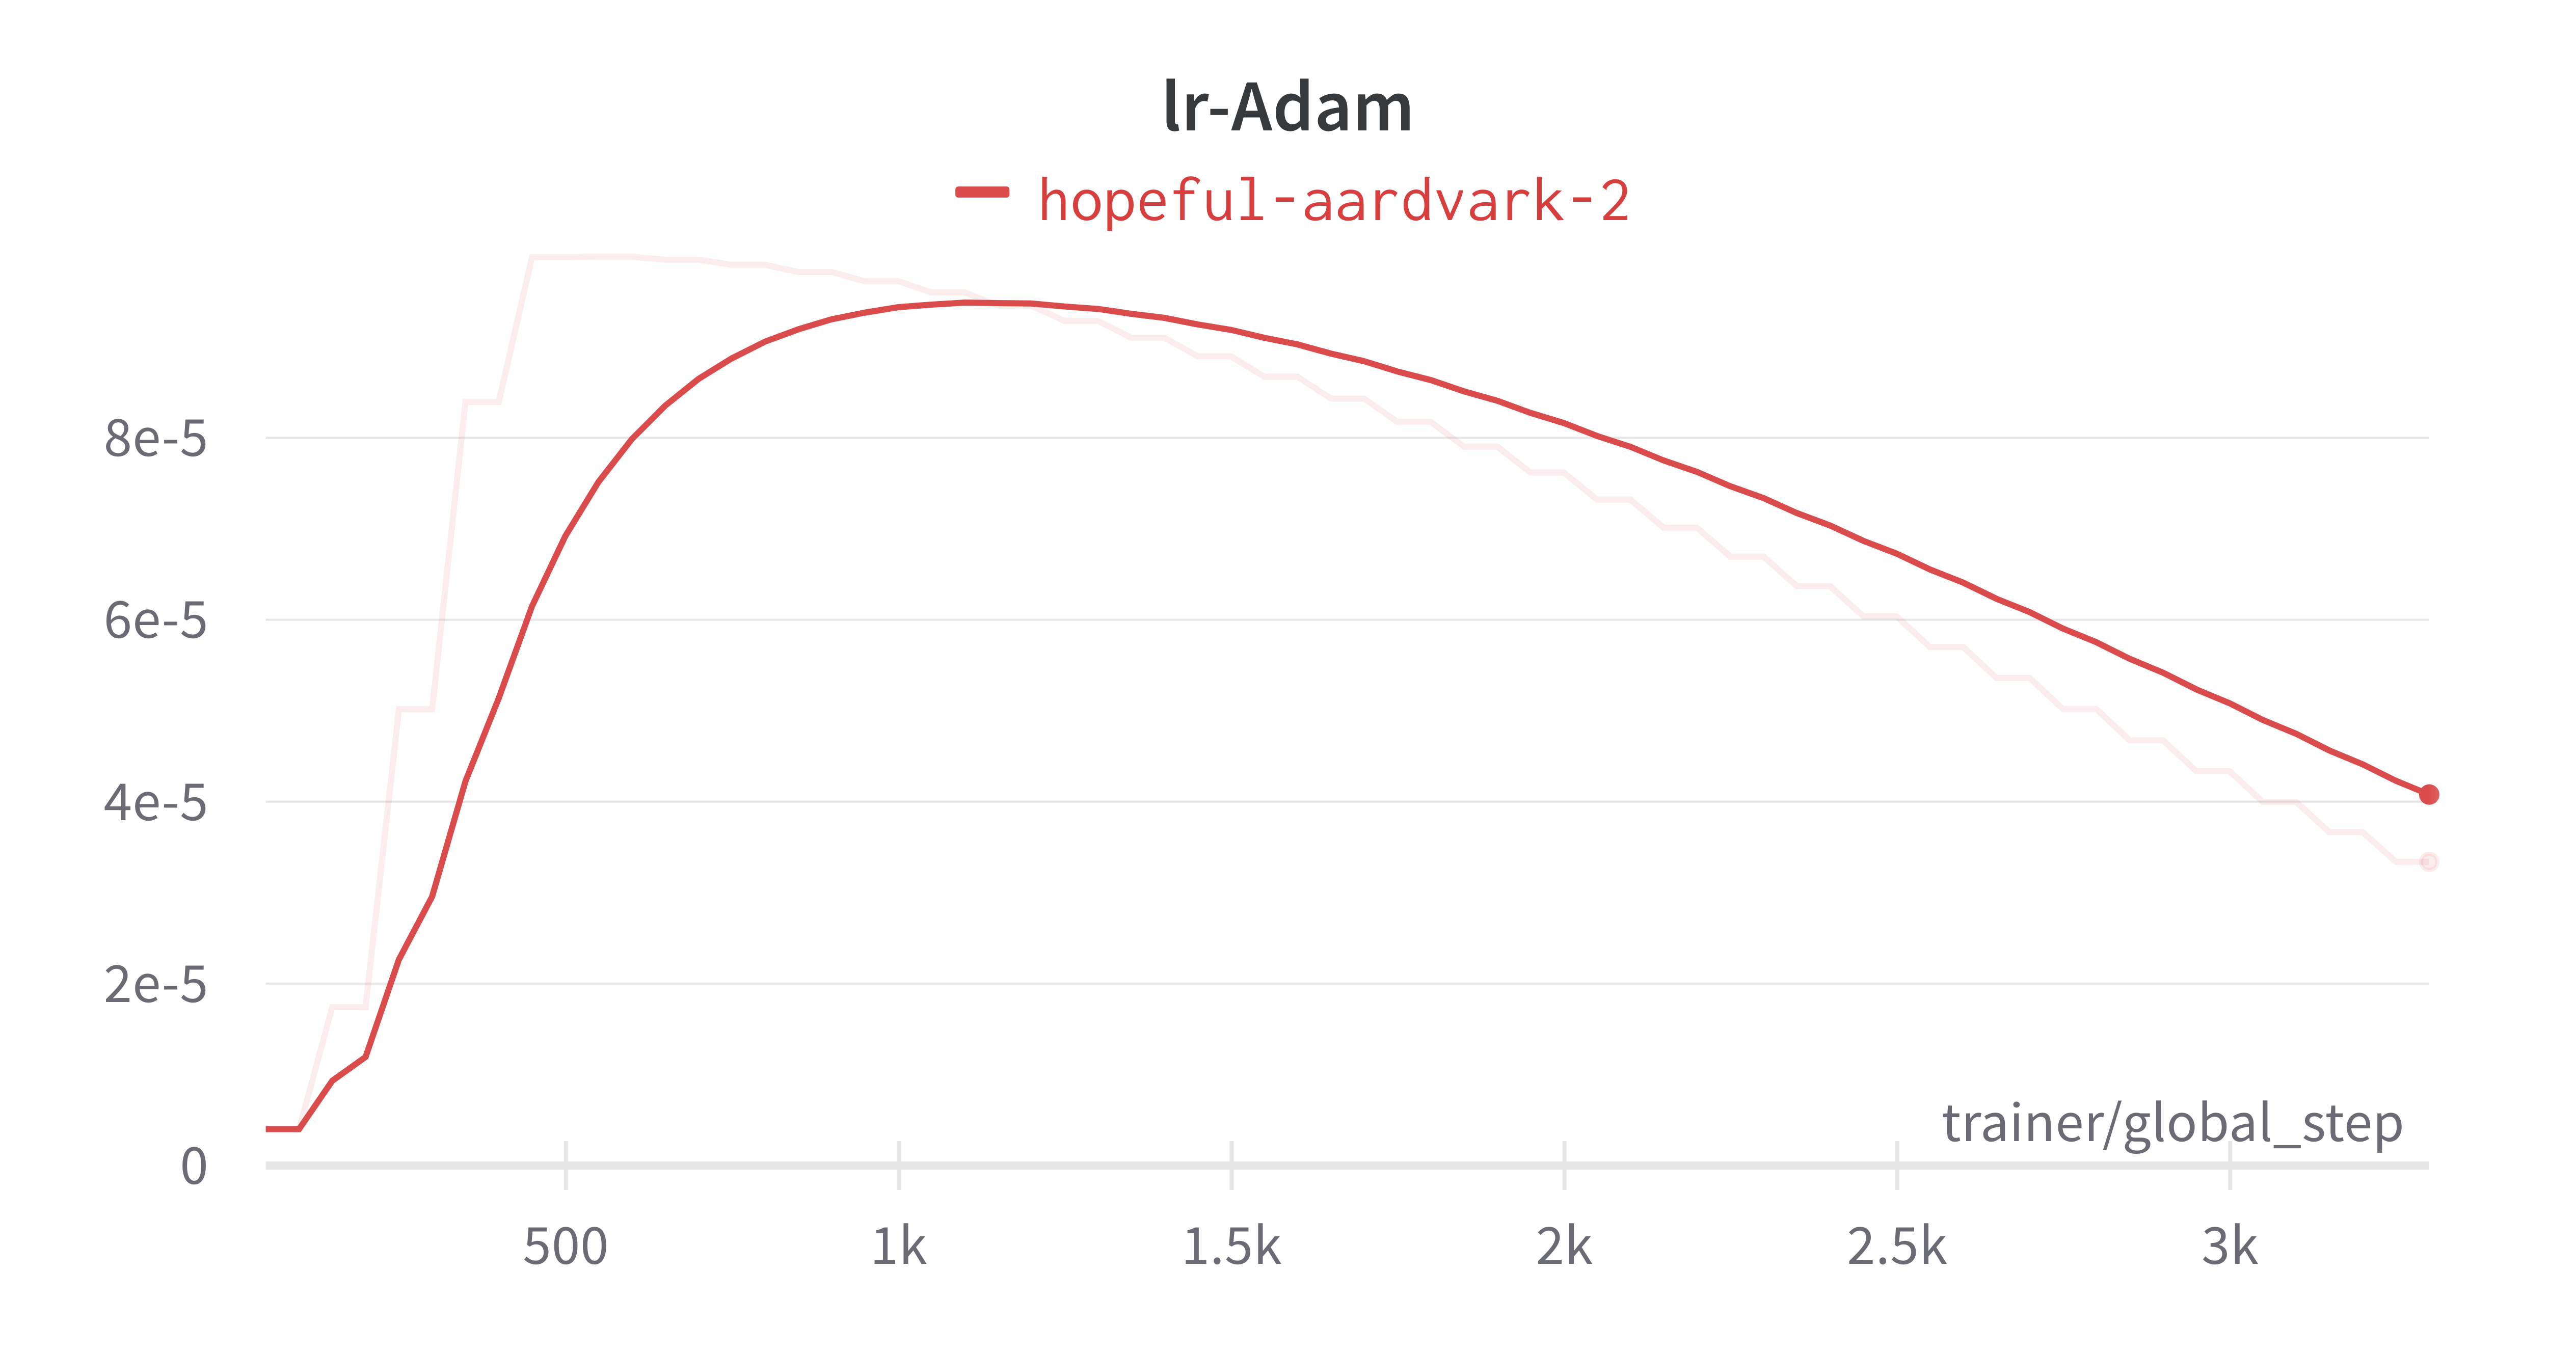
\includegraphics[width=\textwidth]{multitask-lr.png}
        \caption{Uczenie wielozadaniowe.}
        % \label{fig:rozklad-40klas-seg}
    \end{subfigure}
    \caption[]{One cycle learning rate scheduler policy}
    \label{fig:one-cycle-policy}
\end{figure}
\subsection{Wyniki}

\begin{table}[]
    \centering
    \begin{tabular}{c|cc}
        zadanie/{[}\%{]} & Acc jednozadaniowe & Acc wielozadaniowe \\ \hline
        segmentacja      & 67.87               & 67.48  \footnotesize{\textbf{$-$0.39}}        \\
        klasyfikacja     & 65.50               & 67.45  \footnotesize{\textbf{+1.95}}        \\ \hline
    średnia          & 66.69               & 67.47  \footnotesize{\textbf{+0.78}}       
\end{tabular}
\caption{Porównanie dokładności dla uczenia jedno- i wielozadaniowe.}
\label{tab:acc-por}
\end{table}

\begin{figure}[ht!]
    \centering
    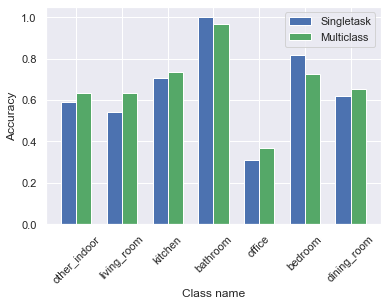
\includegraphics[width=0.75\textwidth]{scene_comp.png}
    \caption{Porównanie dokładności dla każdej z klas w zadaniu klasyfikacji pomieszczeń}
    \label{fig:scene_comp}
\end{figure}

\begin{figure}[ht!]
    \centering
    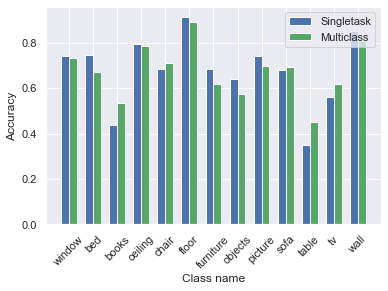
\includegraphics[width=0.75\textwidth]{seg_comp.png}
    \caption{Porównanie dokładności dla każdej z klas w zadaniu segmentacji semantycznej}
    \label{fig:seg_comp}
\end{figure}
Ucznie wielozadaniowe w rozważanym przypadku nieznacznie poprawia wyniki sieci (tab. \ref{tab:acc-por}). Dla zadania segmentacji semantycznej otrzymujemy spadek jakości o 0.39 punkta procentowego. Zadanie klasyfikacji poprawia się o 1.95 p.p. w porównaniu z uczeniem jednozadaniowym. Ostatecznie otrzymujemy zysk na poziomie 0.78 punkta procentego na średniej z zadań. Poprawa jest niewielka, jednak jest to dużu sukces biorąc pod uwagę, że mamy do dyspozycji 2 razy mniej parametrów niz w przypadku dwóch osobnych sieci. Przekłada się to bezpośrednio na czas inferencji, który w przypadku robotyki i systemów czasu rzeczywistego jest kluczowy.

Wartym zobaczenia jest fakt, iż uczenie wielozadaniowe poprawia wyniki dla klas które osiągają najsłabsze rezultaty w uczeniu jednozadaniowym. Poprawie ulega klasa office (rys. \ref{fig:scene_comp}) dla klasyfikacji oraz klasy books oraz table (rys. \ref{fig:seg_comp}) dla segmentacji semantycznej. Powodem jest prawdopodbnie mniejsze obciążenie (bias) modelu spowodowane faktem wzajemnej regularyzacji obu zadań w procesie uczenia. Innymi słowy, model ma mniejszą tendencję do przeuczenia.
\newpage % Rozdziały zaczynamy od nowej strony.
\section{Podsumowanie}

-mozna bylo lepiej to zrobic:
    - augmentacja
    - więcej epok
    - regularyzacja smoothingiem
    - regularayzacja weight decay
-zeby w pelni moc ocenic potencjal uczenia wielozadaniwoe nalezaloby spawdzic modele na wielu zbiorach, w razie potrzeby zachowujac przestrzen reprezentacji a dosziflowujac ostatnie warstwy decyzyjbedroomeabedroom
% \newpage % Rozdziały zaczynamy od nowej strony.
\section{Praefatio}
\lipsum[1] \cite{goossens93}
\begin{figure}[!h]
    \label{fig:tradycyjne-logo-pw}
    \centering 
\includegraphics[width=0.5\linewidth]{logopw.png}
    \caption{Tradycyjne godło Politechniki Warszawskiej}
\end{figure}
\lipsum[2-3]
\begin{figure}[!h]
	\label{fig:nowe-logo-pw}
	\centering 
\includegraphics[width=0.5\linewidth]{logopw2.png}
	\caption{Współczesne logo Politechniki Warszawskiej}
\end{figure}
\lipsum[4-6]
         % Wygodnie jest trzymać każdy rozdział w osobnym pliku.
% \newpage % Rozdziały zaczynamy od nowej strony.
\section{De Finibus Bonorum et Malorum}
\lipsum[1] Lorem ipsum dolor sit amet\footnote{Lorem ipsum dolor sit amet, consectetur adipiscing elit, sed do eiusmod tempor incididunt ut labore et dolore magna aliqua. Ut enim ad minim veniam, quis nostrud exercitation ullamco laboris nisi ut aliquip ex ea commodo consequat.}.
\begin{align*}
    E & = mc^2 \\
    y & = ax^2 + bx + c
\end{align*}

\lipsum[3]

\begin{align}
\begin{bmatrix}
    1 & 0 & 0 \\
    0 & 2 & 0 \\
    0 & 0 & 3
\end{bmatrix} \cdot
\begin{bmatrix}
    4 \\ 5 \\ 6
\end{bmatrix} =
\begin{bmatrix}
    4 \\ 10 \\ 18
\end{bmatrix}
\end{align}

\lipsum[4] Lorem ipsum dolor sit amet, consectetur adipiscing elit, sed do eiusmod tempor incididunt ut labore et dolore magna aliqua \cite{szczypiorski2015}, \cite{duqu2011}, \cite{shs2015}, \cite{wozniak2018}, \cite{dcp19}.

\subsection{Critique of Pure Reason}
\kant[1]

\begin{table}[!h] \label{tab:tabela1} \centering
\caption{Przykładowa tabela.}
\begin{tabular} {| c | c | r |} \hline
    Kolumna 1 & Kolumna 2 & Liczba \\ \hline\hline
    cell1 & cell2 & 60 \\ \hline
    cell4 & cell5 & 43 \\ \hline
    cell7 & cell8 & 20,45 \\ \hline
    \multicolumn{2}{|r|}{Suma:} & 123,45 \\ \hline
\end{tabular}
\end{table}

\kant[2]

\begin{longtable}{| c | m{0.58\linewidth} | r | m{0.1\linewidth} |}
    \caption{Tabela wielostronicowa.} \\
    \hline
    Lp & \multicolumn{1}{c|}{Treść} & \multicolumn{1}{c|}{Kwota} & \multicolumn{1}{m{0.1\linewidth}|}{Wariant opłaty} \\ \hline\hline \endfirsthead

    \endfoot
    \hline \endlastfoot

    1 & Lorem ipsum dolor sit amet, consectetur adipiscing elit, sed do eiusmod tempor incididunt ut labore et dolore magna aliqua. & 111 111,11 zł & \multicolumn{1}{c|}{WAR1} \\ \hline
    2 & Lorem ipsum dolor sit amet, consectetur adipiscing elit, sed do eiusmod tempor incididunt ut labore et dolore magna aliqua. & 22 222,22 zł & \multicolumn{1}{c|}{WAR1} \\ \hline
    3 & Lorem ipsum dolor sit amet, consectetur adipiscing elit, sed do eiusmod tempor incididunt ut labore et dolore magna aliqua. & 33 333,33 zł & \multicolumn{1}{c|}{WAR1} \\ \hline
    4 & Lorem ipsum dolor sit amet, consectetur adipiscing elit, sed do eiusmod tempor incididunt ut labore et dolore magna aliqua. & 444 444,44 zł & \multicolumn{1}{c|}{WAR1} \\ \hline
    5 & Lorem ipsum dolor sit amet, consectetur adipiscing elit, sed do eiusmod tempor incididunt ut labore et dolore magna aliqua. & 55 555,55 zł & \multicolumn{1}{c|}{WAR1} \\ \hline
    6 & Lorem ipsum dolor sit amet, consectetur adipiscing elit, sed do eiusmod tempor incididunt ut labore et dolore magna aliqua. & 66 666,66 zł & \multicolumn{1}{c|}{WAR1} \\ \hline
    7 & Lorem ipsum dolor sit amet, consectetur adipiscing elit, sed do eiusmod tempor incididunt ut labore et dolore magna aliqua. & 777 777,77 zł & \multicolumn{1}{c|}{WAR1} \\ \hline
    8 & Lorem ipsum dolor sit amet, consectetur adipiscing elit, sed do eiusmod tempor incididunt ut labore et dolore magna aliqua. & 8 888,88 zł & \multicolumn{1}{c|}{WAR1} \\ \hline
    9 & Lorem ipsum dolor sit amet, consectetur adipiscing elit, sed do eiusmod tempor incididunt ut labore et dolore magna aliqua. & 999 999,99 zł & \multicolumn{1}{c|}{WAR1} \\ \hline
    10 & Lorem ipsum dolor sit amet, consectetur adipiscing elit, sed do eiusmod tempor incididunt ut labore et dolore magna aliqua. & 111 111,11 zł & \multicolumn{1}{c|}{WAR2} \\ \hline
    11 & Lorem ipsum dolor sit amet, consectetur adipiscing elit, sed do eiusmod tempor incididunt ut labore et dolore magna aliqua. & 22 222,22 zł & \multicolumn{1}{c|}{WAR2} \\ \hline
    12 & Lorem ipsum dolor sit amet, consectetur adipiscing elit, sed do eiusmod tempor incididunt ut labore et dolore magna aliqua. & 33 333,33 zł & \multicolumn{1}{c|}{WAR2} \\ \hline
    13 & Lorem ipsum dolor sit amet, consectetur adipiscing elit, sed do eiusmod tempor incididunt ut labore et dolore magna aliqua. & 444 444,44 zł & \multicolumn{1}{c|}{WAR2} \\ \hline
    14 & Lorem ipsum dolor sit amet, consectetur adipiscing elit, sed do eiusmod tempor incididunt ut labore et dolore magna aliqua. & 55 555,55 zł & \multicolumn{1}{c|}{WAR2} \\ \hline
    15 & Lorem ipsum dolor sit amet, consectetur adipiscing elit, sed do eiusmod tempor incididunt ut labore et dolore magna aliqua. & 66 666,66 zł & \multicolumn{1}{c|}{WAR2} \\ \hline
    & \multicolumn{1}{r|}{\textbf{Suma:}} & \textbf{7 777 777,77 zł} &
    \label{table:koszty}
\end{longtable}
\kant[4]

\subsection{Categorical Imperative}
\subsubsection{Deontological Ethics}
As any dedicated reader can clearly see, the Ideal of practical reason is a representation of, as far as I know, the things in themselves; as I have shown elsewhere, the phenomena should only be used as a canon for our understanding:
% Parametr label ustawia symbol, a leftmargin - wielkość wcięcia.
% Domyślny układ to [---] bez wcięcia, bo tak pan Marcin Woliński powiedział;
% ale ja nie polecam. // AB
\begin{itemize}
    \item Item 1:
    \begin{itemize}[label=---]
        \item item 1.1;
        \item item 1.2;
        \item item 1.3;
    \end{itemize}
    \item Item 2;
    \item Item 3;
    \item Item 4.
\end{itemize}
\kant[2]

\subsubsection{Consequentialism -- the Ideal of practical reason}
\kant[3]
\begin{enumerate}
    \item Item 1:
    \begin{enumerate}
        \item item 1.1;
        \item item 1.2:
        \begin{enumerate}
            \item item 1.2.1;
            \item item 1.2.2;
        \end{enumerate}
        \item item 1.3;
    \end{enumerate}
    \item Item 2;
    \item Item 3;
    \item Item 4.
\end{enumerate}

\kant[9]

\subsection{G\"odel's ontological proof}
\kant[9] Lorem ipsum dolor sit amet, consectetur adipiscing elit, sed do eiusmod tempor incididunt ut labore et dolore magna aliqua \cite{benzmuller2014}, \cite{goedel95}, \cite{wang97}, \cite{koons2005}.
\begin{assumption} \label{ass:1}
    $ [\![ \ \phi \ ]\!] \Longrightarrow [\![ \ P(\phi); \neg P(\phi) \ ]\!]$
\end{assumption}
\begin{axiom}[Dualność] \label{axiom:1}
    $\neg P(\phi) \Leftrightarrow P(\neg \phi)$, równoważnie $P(\phi) \Leftrightarrow \neg P(\neg \phi)$
\end{axiom}
\begin{axiom}[Całkowitość] \label{axiom:2}
    $ \left( P(\phi) \wedge \forall x: \phi(x) \Rightarrow \psi(x) \right) \Rightarrow P(\psi) $
\end{axiom}
\begin{axiom}[Absolutność] \label{axiom:3}
    $ P(\phi) \Rightarrow \Box P(\phi) $
\end{axiom}
\begin{definition} \label{def:1}
    $ G(x) \Leftrightarrow \forall \phi: \left( P(\phi) \Rightarrow \phi(x) \right) $
\end{definition}
\begin{definition} \label{def:2}
    $ \phi \ ess \ x \Leftrightarrow \phi(x) \wedge \forall \psi \left( \psi(x) \Rightarrow \Box \forall y \left( \phi(y) \Rightarrow \psi(y) \right) \right)  $
\end{definition}
\begin{axiom} \label{axiom:4}
    P(G)
\end{axiom}
\begin{lemma} \label{lemma:1}
    $ P(\phi) \Rightarrow \Diamond \exists x : \phi(x) $
\end{lemma}
\begin{proof}
    Dowód pomijamy, bo jest trywialny :)
\end{proof}
\begin{lemma} \label{lemma:2}
    $ \Diamond \exists x : G(x) $
\end{lemma}
\begin{proof}
    Natychmiastowy wniosek z aksjomatu \ref{axiom:4} i lematu \ref{lemma:1}.
\end{proof}
\begin{lemma} \label{lemma:3}
    $ G(x) \Rightarrow G \ ess \ x $
\end{lemma}
\begin{proof}
    Poprzez podstawienie do definicji \ref{def:2}.
\end{proof}
\begin{definition} \label{def:3}
    $ E(x) \Leftrightarrow \forall \phi \left( \phi \ ess \ x \Rightarrow \Box\ \exists x: \phi(x) \right) $
\end{definition}
\begin{axiom} \label{axiom:5}
    P(E)
\end{axiom}
\begin{theorem}
    $ \Box\ \exists x : G(x) $
\end{theorem}
\begin{proof}
    Na podstawie definicji \ref{def:1}, lematu \ref{lemma:3} i aksjomatu \ref{axiom:5}.
\end{proof}    % Umożliwia to również łatwą migrację do nowej wersji szablonu:
% \newpage % Rozdziały zaczynamy od nowej strony.
\section{Code listings}

\lipsum[10]
% \addmargin pozwala na wcięcie kodu od lewej (tutaj: 6mm).
% Wcięcie pomaga ustawić kod tak, 
% aby numery linii nie były za bardzo na lewo. 
% Druga liczba oznacza wcięcie od prawej. 
\begin{addmargin}[6mm]{0mm}
\begin{lstlisting}[
    language=HTML,
    numbers=left,
    firstnumber=1,
    caption={\emph{Hello world} w HTML},
    aboveskip=0pt
]
<html>
  <head>
    <title>Hello world!</title>
  </head>
  <body>
    Hello world!
  </body>
</html>
\end{lstlisting}
\end{addmargin}

\lipsum[11]
% Dla dłuższych numerów linii
% potrzebne jest większe wcięcie.
\begin{addmargin}[10mm]{0mm}
\begin{lstlisting}[
    language=C++,
    numbers=left,
    firstnumber=147,
    caption={Generowanie sekwencji Collatza w języku C++},
    aboveskip=0pt
]
class Collatz {
  private:
    unsigned current_val_;
    void update_val() {
        if( current_val_ % 2 == 0 )
            current_val_ /= 2;
        else
            current_val_ = current_val_ * 3 + 1;
    }

  public:
    explicit Collatz(unsigned initial_value) : 
        current_val_(initial_value) {}
    void print_sequence() {
        unsigned i = 1;
        while( current_val_ > 1 ) {
            std::cout
                << "val " << i << " = " << current_val_
                << std::endl;
            update_val(); ++i;
        }
    }
};

int main() {
  // prints Collatz seqence, starting from 194375
  Collatz seq(194375);
  seq.print_sequence();
  return 0;
}
\end{lstlisting}
\end{addmargin}

\lipsum[12]
 % wystarczy podmienić swoje pliki main.tex i eiti-thesis.cls
%                             % na nowe wersje, a cały tekst pracy pozostaje nienaruszony.
% \newpage % Rozdziały zaczynamy od nowej strony
% \section{Summatio}          % Można też pisać rozdziały w jednym pliku.
% \lipsum[5-10]

%--------------------------------------------
% Literatura
%--------------------------------------------
\cleardoublepage % Zaczynamy od nieparzystej strony
\printbibliography

%--------------------------------------------
% Spisy (opcjonalne)
%--------------------------------------------
\newpage
\pagestyle{plain}

% Wykaz symboli i skrótów.
% Pamiętaj, żeby posortować symbole alfabetycznie
% we własnym zakresie. Ponieważ mało kto używa takiego wykazu,
% uznałem, że robienie automatycznie sortowanej listy
% na poziomie LaTeXa to za duży overkill.
% Makro \acronymlist generuje właściwy tytuł sekcji,
% w zależności od języka.
% Makro \acronym dodaje skrót/symbol do listy,
% zapewniając podstawowe formatowanie.
% //AB
% \vspace{0.8cm}
% \acronymlist
% \acronym{EiTI}{Wydział Elektroniki i Technik Informacyjnych}
% \acronym{PW}{Politechnika Warszawska}
% \acronym{WEIRD}{ang. \emph{Western, Educated, Industrialized, Rich and Democratic}}

\listoffigurestoc     % Spis rysunków.
\vspace{1cm}          % vertical space
\listoftablestoc      % Spis tabel.
% \vspace{1cm}          % vertical space
% \listofappendicestoc  % Spis załączników

% Załączniki
% \newpage
% \appendix{Nazwa załącznika 1}
% \lipsum[1-8]

% \newpage
% \appendix{Nazwa załącznika 2}
% \lipsum[1-4]

% Używając powyższych spisów jako szablonu,
% możesz tu dodać swój własny wykaz bądź listę,
% np. spis algorytmów.

\end{document} % Dobranoc.
